% Created 2015-05-29 fr. 13:37
\documentclass[presentation]{beamer}
\usepackage[utf8]{inputenc}
\usepackage[T1]{fontenc}
\usepackage{fixltx2e}
\usepackage{graphicx}
\usepackage{longtable}
\usepackage{float}
\usepackage{wrapfig}
\usepackage{rotating}
\usepackage[normalem]{ulem}
\usepackage{amsmath}
\usepackage{textcomp}
\usepackage{marvosym}
\usepackage{wasysym}
\usepackage{amssymb}
\usepackage{capt-of}
\usepackage{hyperref}
\tolerance=1000
\usepackage{minted}
\usepackage{color}
\usepackage{listings}
\usepackage{minted}
\usepackage{xcolor}
\useoutertheme[subsection=false]{smoothbars}
\usecolortheme{whale}
\useinnertheme{rectangles}
\setbeamertemplate{footline}[frame number]
\usemintedstyle{emacs}
\usepackage[natbib=true,uniquelist=false,bibstyle=authoryear-comp,citestyle=authoryear-comp,sorting=nyt,sortcase=false,sortcites=true,minbibnames=6,maxbibnames=6,maxcitenames=2,hyperref=false,backref=false,backend=bibtex,isbn=false,url=false,doi=false,eprint=false,firstinits=true,terseinits=true,dashed=false,uniquename=false,uniquelist=false]{biblatex}
\addbibresource{/home/alj/Dropbox.personal/Dropbox/Literature/CompleteLiterature.bib}
\usepackage{tikz,graphics,graphicx}
\usetikzlibrary{decorations.shapes,arrows,decorations.pathreplacing,decorations.pathmorphing,backgrounds}
\usetikzlibrary{decorations.pathmorphing}
\usetikzlibrary{shapes.geometric}
% Centering frame titles:
\makeatletter
\long\def\beamer@@frametitle[#1]#2{%
\beamer@ifempty{#2}{}{%
\gdef\insertframetitle{
\centering{#2\ifnum\beamer@autobreakcount>0\relax{}
\space\usebeamertemplate*{frametitle continuation}\fi}}%
\gdef\beamer@frametitle{#2}%
\gdef\beamer@shortframetit   le{#1}%
}%
}
\makeatother
% Getting the frametitles in bold
\setbeamerfont{frametitle}{series=\bfseries}
\usetheme{default}
\author{Alexander Jueterbock}
\date{2015-05-30}
\title{Non-model species and RAD-sequencing}
\begin{document}

\maketitle




\begin{frame}[label=sec-0-0-1]{RAD-Seq is a young and successful NGS method}
\begin{center}


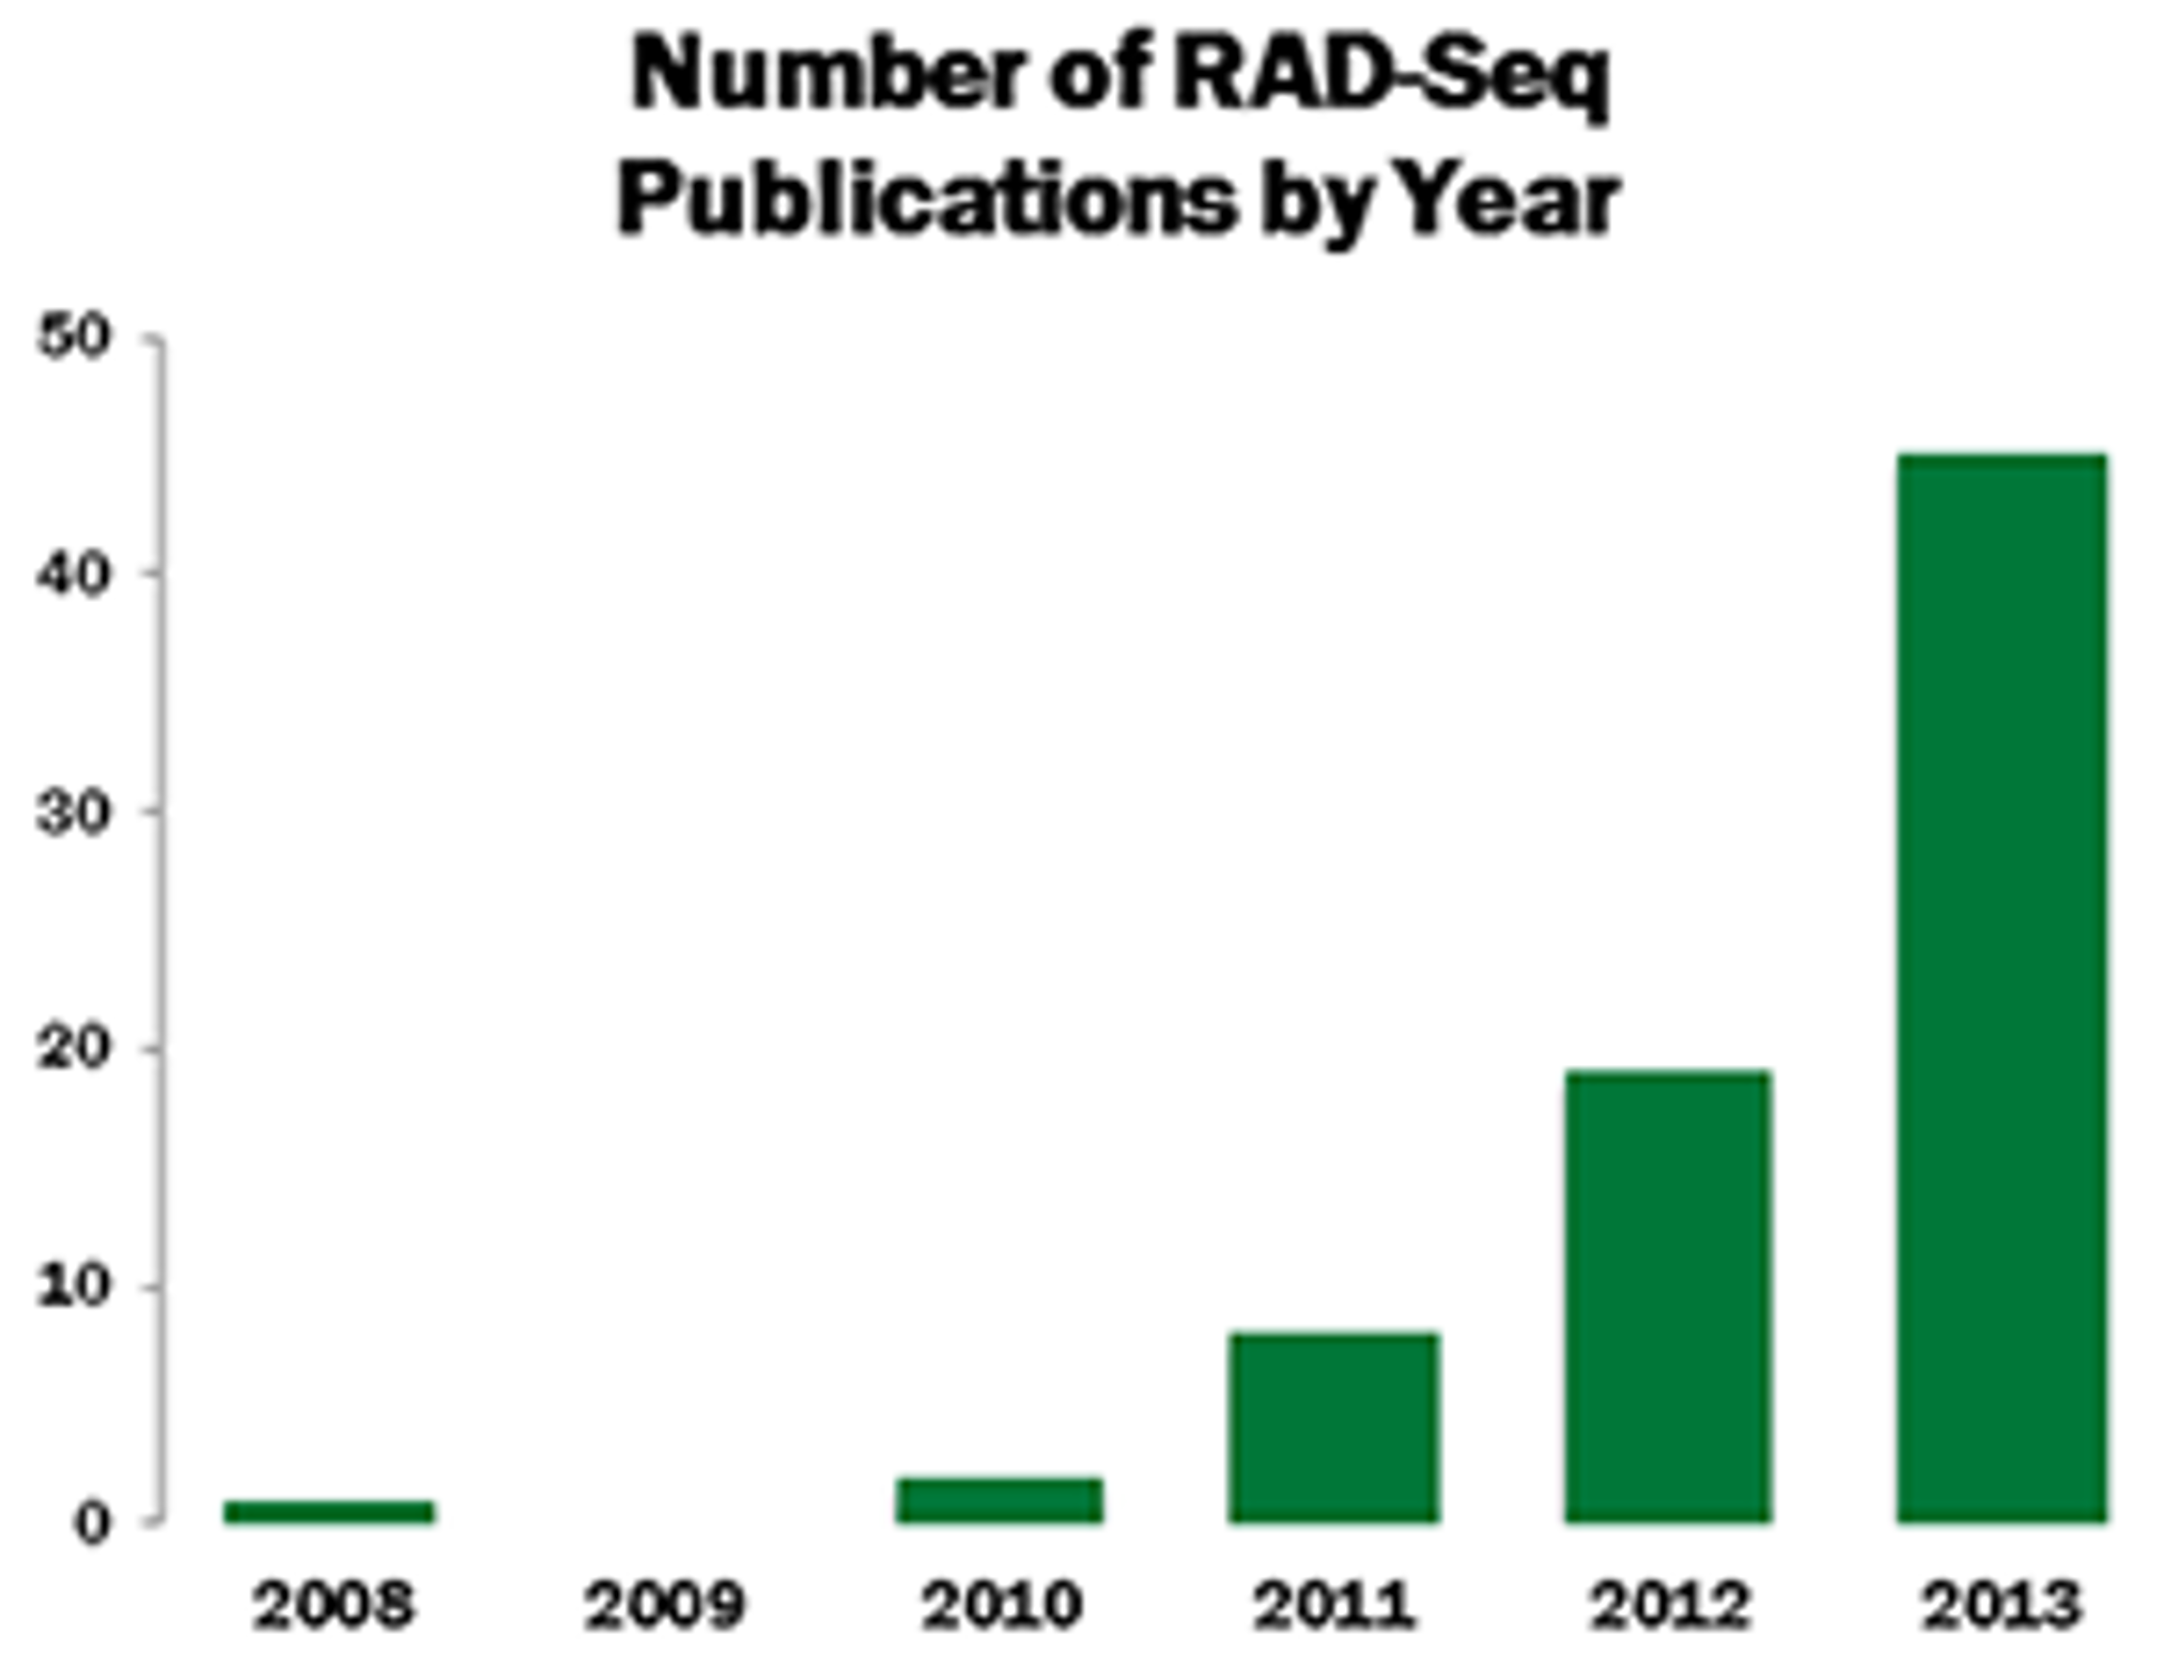
\includegraphics[width=7cm]{RADSeqPublications.png}

\tiny{source: http://ngs-expert.com/2013/11/26/rad-seq-publications-in-2013/}
\end{center}
\end{frame}

\begin{frame}[label=sec-0-0-2]{Reductive \emph{de novo} genome sequencing and SNP identification}
\begin{itemize}
\item RAD-Seq of the sunflower genome (Illumina)
\begin{itemize}
\item 44.7M reads (PE:40bpx80bp)
\end{itemize}
\item \emph{De novo} assembly of ca. 15.2 Mb 
in >42,000 contigs
\item Identified >94,000 putative SNPs across six lines
\end{itemize}
\begin{center}

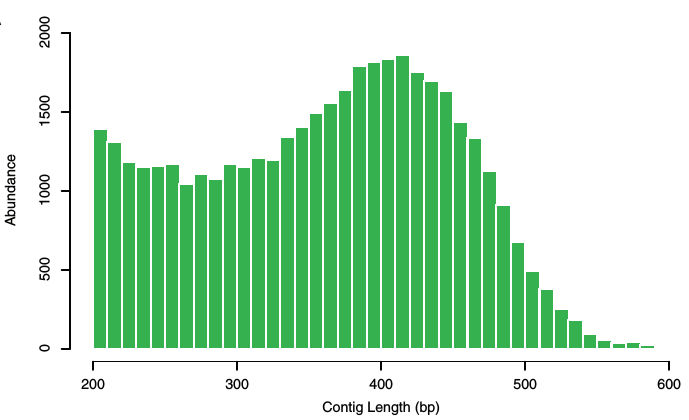
\includegraphics[width=8cm]{Pegadarju2013Fig3a.png}


\tiny{\citep{Pegadaraju2013}}
\end{center}
\end{frame}





\begin{frame}[label=sec-0-0-3]{Genome-wide association study (GWAS)}
\begin{itemize}
\item No reference genome previously available
\item identified >100,000 SNPs across 138 genotypes
\item Related SNPs to 17 phenotypic traits in a field trial
\item Increasing flexibility and speed of crop breeding
\end{itemize}


\begin{figure}[htb]
\centering
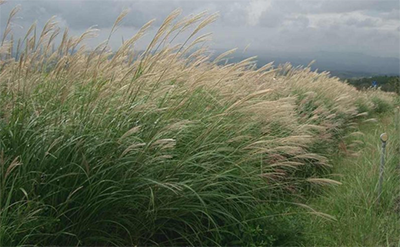
\includegraphics[width=5.5cm]{miscanthus.png}
\caption{\emph{Miscanthus sinensis}}
\end{figure}




\begin{center}
\tiny{source: http://ngs-expert.com/2013/11/26/rad-seq-publications-in-2013/}
\tiny{\citep{Slavov2014}}
\end{center}
\end{frame}



\begin{frame}[label=sec-0-0-4]{Population genomics and parallel adaptive differentiation in threespine sticklebacks}
\begin{itemize}
\item Reference genome available
\item >45,000 SNPs across 100 individuals ('genotyping by sequencing')
\item Consistent signatures of selection between two oceanic and three
freshwater populations
\item Identified 31 candidate genes of evolutionary significance
\end{itemize}


\begin{figure}[htb]
\centering
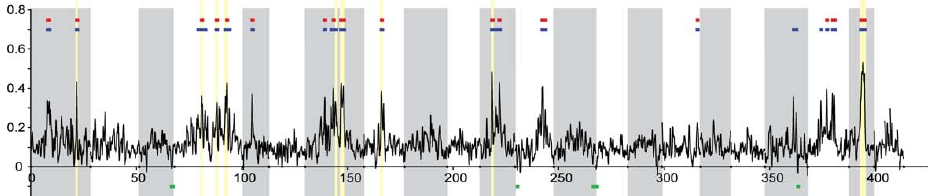
\includegraphics[width=10cm]{Hohenlohe2010Fig6e.png}
\caption{F\(_{\text{ST}}\) for SNPs in sliding windows across the genome between oceanic and freshwater populations}
\end{figure}


\begin{center}
\tiny{\citep{Hohenlohe2010}}
\end{center}
\end{frame}



\begin{frame}[label=sec-0-0-5]{Purpose of RAD-seq}
\begin{itemize}
\item Genome-reduction method to fragments adjacent to restriction enzyme
recognition sites.
\item High-throughput genotyping of populations (using barcoding) at
relatively low cost.
\item Makes genome-scale population genetic studies possible for non-model
species lacking a reference genome.
\end{itemize}
\end{frame}

\section{RAD-Seq}
\label{sec-1}

\subsection{RAD-Seq}
\label{sec-1-1}


\begin{frame}[label=sec-1-1-1]{Original RAD-Seq protocol}
\begin{itemize}
\item Developed by \citep{Miller2007, Baird2008}.
\item DNA fragments adjacent to restriction enzyme recognition sites
\end{itemize}


\definecolor{redd}{rgb}{0.8431373,0.09803922,0.1098039}

\begin{center}
\begin{figure}[htb]
\setlength{\belowcaptionskip}{-1cm}
\scalebox{1}{
\begin{tikzpicture}
\draw [redd, line width=0.2cm] (0cm,0cm) --  (0.3cm,0cm);
\draw [redd, line width=0.2cm] (0cm,-0.5cm) --  (0.3cm,-0.5cm);
\draw [redd, line width=0.2cm] (0cm,-1cm) --  (0.3cm,-1cm);
\draw [redd, line width=0.2cm] (0cm,-1.5cm) --  (0.3cm,-1.5cm);

\draw [gray, line width=0.2cm] (0.3cm,0cm) --  (10cm,0cm);
\draw [gray, line width=0.2cm] (0.3cm,-0.5cm) --  (4cm,-0.5cm);
\draw [gray, line width=0.2cm] (0.3cm,-1cm) --  (6cm,-1cm);
\draw [gray, line width=0.2cm] (0.3cm,-1.5cm) --  (7.5cm,-1.5cm);
\node [color=redd] at (1cm,-2.5cm) {5' GAATTC 3'};
\node [color=redd] at (1cm,-3cm) {3' CTTAAG 5'};
\node [color=black] at (5cm,-2.75cm) {EcoRI recognition site};
\node [isosceles triangle, draw, rotate=270,scale=0.4,fill=redd!50!black] at (0.5cm,-2cm) {}; 
\node [isosceles triangle, draw, rotate=90,scale=0.4,fill=redd!50!black] at (1.5cm,-3.5cm) {}; 

\end{tikzpicture}
} 
\end{figure}
\end{center}
\end{frame}


\begin{frame}[label=sec-1-1-2]{Step 1: cut DNA}
\definecolor{redd}{rgb}{0.8431373,0.09803922,0.1098039}
\begin{center}

\begin{figure}[htb]
\setlength{\belowcaptionskip}{-1cm}
\scalebox{1}{
\begin{tikzpicture}
\draw [redd, line width=0.15cm] (0cm,0cm) --  (0.3cm,0cm);
\draw [gray, line width=0.15cm] (0.3cm,0cm) --  (10cm,0cm);
\draw [redd, line width=0.15cm] (1cm,0cm) --  (1.3cm,0cm);
\draw [redd, line width=0.15cm] (5cm,0cm) --  (5.3cm,0cm);
\draw [redd, line width=0.15cm] (7cm,0cm) --  (7.3cm,0cm);
\draw [redd, line width=0.15cm] (10cm,0cm) --  (10.3cm,0cm);


\node [isosceles triangle, draw, rotate=270,scale=0.1,fill=redd!50!black] at (0.05cm,0.2cm) {}; 
\node [isosceles triangle, draw, rotate=90,scale=0.1,fill=redd!50!black] at (0.25cm,-0.2cm) {}; 

\node [isosceles triangle, draw, rotate=270,scale=0.1,fill=redd!50!black] at (1.05cm,0.2cm) {}; 
\node [isosceles triangle, draw, rotate=90,scale=0.1,fill=redd!50!black] at (1.25cm,-0.2cm) {}; 

\node [isosceles triangle, draw, rotate=270,scale=0.1,fill=redd!50!black] at (5.05cm,0.2cm) {}; 
\node [isosceles triangle, draw, rotate=90,scale=0.1,fill=redd!50!black] at (5.25cm,-0.2cm) {}; 

\node [isosceles triangle, draw, rotate=270,scale=0.1,fill=redd!50!black] at (7.05cm,0.2cm) {}; 
\node [isosceles triangle, draw, rotate=90,scale=0.1,fill=redd!50!black] at (7.25cm,-0.2cm) {}; 

\node [isosceles triangle, draw, rotate=270,scale=0.1,fill=redd!50!black] at (10.05cm,0.2cm) {}; 
\node [isosceles triangle, draw, rotate=90,scale=0.1,fill=redd!50!black] at (10.25cm,-0.2cm) {}; 




\begin{scope}[yshift=-1cm]
\draw [redd, line width=0.15cm] (0cm,-0.5cm) --  (0.3cm,-0.5cm);
\draw [gray, line width=0.15cm] (0.3cm,-0.5cm) --  (1cm,-0.5cm);
\draw [redd, line width=0.15cm] (1cm,-0.5cm) --  (1.3cm,-0.5cm);

\draw [redd, line width=0.15cm] (0cm,-1cm) --  (0.3cm,-1cm);
\draw [gray, line width=0.15cm] (0.3cm,-1cm) --  (5cm,-1cm);
\draw [redd, line width=0.15cm] (5cm,-1cm) --  (5.3cm,-1cm);

\draw [redd, line width=0.15cm] (0cm,-1.5cm) --  (0.3cm,-1.5cm);
\draw [gray, line width=0.15cm] (0.3cm,-1.5cm) --  (2cm,-1.5cm);
\draw [redd, line width=0.15cm] (2cm,-1.5cm) --  (2.3cm,-1.5cm);


\draw [redd, line width=0.15cm] (0cm,-2cm) --  (0.3cm,-2cm);
\draw [gray, line width=0.15cm] (0.3cm,-2cm) --  (3cm,-2cm);
\draw [redd, line width=0.15cm] (3cm,-2cm) --  (3.3cm,-2cm);
\end{scope}


\end{tikzpicture}
}
\end{figure}
\end{center}
\begin{itemize}
\item Note: Bias in GC content of restriction site samples the genome
non-randomly
\end{itemize}
\end{frame}

\begin{frame}[label=sec-1-1-3]{Step 2: ligate P1 adapter}


\definecolor{redd}{rgb}{0.8431373,0.09803922,0.1098039}
\definecolor{barcode}{rgb}{0.6352941,0.8588235,0.9176471}
\definecolor{sequencingprimer}{rgb}{0.9882353,0.5529412,0.3490196}
\definecolor{amplificationprimer}{rgb}{0.2705882,0.4588235,0.7058824}

\begin{center}
\begin{figure}[htb]
\setlength{\belowcaptionskip}{-1cm}
\scalebox{1}{
\begin{tikzpicture}



\draw [amplificationprimer, line width=0.15cm] (-0.45cm,-0.5cm) --  (-0.3cm,-0.5cm);
\draw [sequencingprimer, line width=0.15cm] (-0.3cm,-0.5cm) --  (-0.15cm,-0.5cm);
\draw [barcode, line width=0.15cm] (-0.15cm,-0.5cm) --  (0cm,-0.5cm);

\draw [amplificationprimer, line width=0.15cm] (-0.45cm,-1cm) --  (-0.3cm,-1cm);
\draw [sequencingprimer, line width=0.15cm] (-0.3cm,-1cm) --  (-0.15cm,-1cm);
\draw [barcode, line width=0.15cm] (-0.15cm,-1cm) --  (0cm,-1cm);

\draw [amplificationprimer, line width=0.15cm] (-0.45cm,-1.5cm) --  (-0.3cm,-1.5cm);
\draw [sequencingprimer, line width=0.15cm] (-0.3cm,-1.5cm) --  (-0.15cm,-1.5cm);
\draw [barcode, line width=0.15cm] (-0.15cm,-1.5cm) --  (0cm,-1.5cm);

\draw [amplificationprimer, line width=0.15cm] (-0.45cm,-2cm) --  (-0.3cm,-2cm);
\draw [sequencingprimer, line width=0.15cm] (-0.3cm,-2cm) --  (-0.15cm,-2cm);
\draw [barcode, line width=0.15cm] (-0.15cm,-2cm) --  (0cm,-2cm);




\draw [amplificationprimer, line width=0.15cm] (1.6cm,-0.5cm) --  (1.75cm,-0.5cm);
\draw [sequencingprimer, line width=0.15cm] (1.45cm,-0.5cm) --  (1.6cm,-0.5cm);
\draw [barcode, line width=0.15cm] (1.3cm,-0.5cm) --  (1.45cm,-0.5cm);

\draw [amplificationprimer, line width=0.15cm] (5.6cm,-1cm) --  (5.75cm,-1cm);
\draw [sequencingprimer, line width=0.15cm] (5.45cm,-1cm) --  (5.6cm,-1cm);
\draw [barcode, line width=0.15cm] (5.3cm,-1cm) --  (5.45cm,-1cm);

\draw [amplificationprimer, line width=0.15cm] (2.6cm,-1.5cm) --  (2.75cm,-1.5cm);
\draw [sequencingprimer, line width=0.15cm] (2.45cm,-1.5cm) --  (2.6cm,-1.5cm);
\draw [barcode, line width=0.15cm] (2.3cm,-1.5cm) --  (2.45cm,-1.5cm);

\draw [amplificationprimer, line width=0.15cm] (3.6cm,-2cm) --  (3.75cm,-2cm);
\draw [sequencingprimer, line width=0.15cm] (3.45cm,-2cm) --  (3.6cm,-2cm);
\draw [barcode, line width=0.15cm] (3.3cm,-2cm) --  (3.45cm,-2cm);

\draw [redd, line width=0.15cm] (0cm,-0.5cm) --  (0.3cm,-0.5cm);
\draw [gray, line width=0.15cm] (0.3cm,-0.5cm) --  (1cm,-0.5cm);
\draw [redd, line width=0.15cm] (1cm,-0.5cm) --  (1.3cm,-0.5cm);

\draw [redd, line width=0.15cm] (0cm,-1cm) --  (0.3cm,-1cm);
\draw [gray, line width=0.15cm] (0.3cm,-1cm) --  (5cm,-1cm);
\draw [redd, line width=0.15cm] (5cm,-1cm) --  (5.3cm,-1cm);

\draw [redd, line width=0.15cm] (0cm,-1.5cm) --  (0.3cm,-1.5cm);
\draw [gray, line width=0.15cm] (0.3cm,-1.5cm) --  (2cm,-1.5cm);
\draw [redd, line width=0.15cm] (2cm,-1.5cm) --  (2.3cm,-1.5cm);


\draw [redd, line width=0.15cm] (0cm,-2cm) --  (0.3cm,-2cm);
\draw [gray, line width=0.15cm] (0.3cm,-2cm) --  (3cm,-2cm);
\draw [redd, line width=0.15cm] (3cm,-2cm) --  (3.3cm,-2cm);




\draw [amplificationprimer, line width=0.3cm] (-0.45cm,-3.5cm) --  (0cm,-3.5cm);
\draw [sequencingprimer, line width=0.3cm] (0cm,-3.5cm) --  (0.45cm,-3.5cm);
\draw [barcode, line width=0.3cm] (0.45cm,-3.5cm) --  (0.9cm,-3.5cm);

\node [color=amplificationprimer,anchor=west] at (-0.45cm,-4cm) {Amplification primer site};
\node [color=sequencingprimer,anchor=west] at (0cm,-4.7cm) {Sequencing primer site (Illumina-specific)};
\node [color=barcode,anchor=west] at (0.45cm,-5.4cm) {Barcode};



\end{tikzpicture}
}
\end{figure}
\end{center}
\end{frame}

\begin{frame}[label=sec-1-1-4]{Barcoding allows to pool samples}


\definecolor{redd}{rgb}{0.8431373,0.09803922,0.1098039}
\definecolor{barcode}{rgb}{0.6352941,0.8588235,0.9176471}
\definecolor{barcode2}{rgb}{0.498039,1,0}
\definecolor{barcode3}{rgb}{0.6,0.196078,0.8}
\definecolor{barcode4}{rgb}{1,0.843137,0}
\definecolor{sequencingprimer}{rgb}{0.9882353,0.5529412,0.3490196}
\definecolor{amplificationprimer}{rgb}{0.2705882,0.4588235,0.7058824}

\begin{center}
\begin{figure}[htb]
\setlength{\belowcaptionskip}{-1cm}
\scalebox{1}{
\begin{tikzpicture}



\draw [amplificationprimer, line width=0.15cm] (-0.45cm,-0.5cm) --  (-0.3cm,-0.5cm);
\draw [sequencingprimer, line width=0.15cm] (-0.3cm,-0.5cm) --  (-0.15cm,-0.5cm);
\draw [barcode, line width=0.15cm] (-0.15cm,-0.5cm) --  (0cm,-0.5cm);

\draw [amplificationprimer, line width=0.15cm] (-0.45cm,-1cm) --  (-0.3cm,-1cm);
\draw [sequencingprimer, line width=0.15cm] (-0.3cm,-1cm) --  (-0.15cm,-1cm);
\draw [barcode2, line width=0.15cm] (-0.15cm,-1cm) --  (0cm,-1cm);

\draw [amplificationprimer, line width=0.15cm] (-0.45cm,-1.5cm) --  (-0.3cm,-1.5cm);
\draw [sequencingprimer, line width=0.15cm] (-0.3cm,-1.5cm) --  (-0.15cm,-1.5cm);
\draw [barcode3, line width=0.15cm] (-0.15cm,-1.5cm) --  (0cm,-1.5cm);

\draw [amplificationprimer, line width=0.15cm] (-0.45cm,-2cm) --  (-0.3cm,-2cm);
\draw [sequencingprimer, line width=0.15cm] (-0.3cm,-2cm) --  (-0.15cm,-2cm);
\draw [barcode, line width=0.15cm] (-0.15cm,-2cm) --  (0cm,-2cm);

\draw [amplificationprimer, line width=0.15cm] (-0.45cm,-2.5cm) --  (-0.3cm,-2.5cm);
\draw [sequencingprimer, line width=0.15cm] (-0.3cm,-2.5cm) --  (-0.15cm,-2.5cm);
\draw [barcode4, line width=0.15cm] (-0.15cm,-2.5cm) --  (0cm,-2.5cm);

\draw [amplificationprimer, line width=0.15cm] (-0.45cm,-3cm) --  (-0.3cm,-3cm);
\draw [sequencingprimer, line width=0.15cm] (-0.3cm,-3cm) --  (-0.15cm,-3cm);
\draw [barcode2, line width=0.15cm] (-0.15cm,-3cm) --  (0cm,-3cm);




\draw [amplificationprimer, line width=0.15cm] (1.6cm,-0.5cm) --  (1.75cm,-0.5cm);
\draw [sequencingprimer, line width=0.15cm] (1.45cm,-0.5cm) --  (1.6cm,-0.5cm);
\draw [barcode, line width=0.15cm] (1.3cm,-0.5cm) --  (1.45cm,-0.5cm);

\draw [amplificationprimer, line width=0.15cm] (5.6cm,-1cm) --  (5.75cm,-1cm);
\draw [sequencingprimer, line width=0.15cm] (5.45cm,-1cm) --  (5.6cm,-1cm);
\draw [barcode2, line width=0.15cm] (5.3cm,-1cm) --  (5.45cm,-1cm);

\draw [amplificationprimer, line width=0.15cm] (2.6cm,-1.5cm) --  (2.75cm,-1.5cm);
\draw [sequencingprimer, line width=0.15cm] (2.45cm,-1.5cm) --  (2.6cm,-1.5cm);
\draw [barcode3, line width=0.15cm] (2.3cm,-1.5cm) --  (2.45cm,-1.5cm);

\draw [amplificationprimer, line width=0.15cm] (3.6cm,-2cm) --  (3.75cm,-2cm);
\draw [sequencingprimer, line width=0.15cm] (3.45cm,-2cm) --  (3.6cm,-2cm);
\draw [barcode, line width=0.15cm] (3.3cm,-2cm) --  (3.45cm,-2cm);

\draw [amplificationprimer, line width=0.15cm] (4.6cm,-2.5cm) --  (4.75cm,-2.5cm);
\draw [sequencingprimer, line width=0.15cm] (4.45cm,-2.5cm) --  (4.6cm,-2.5cm);
\draw [barcode4, line width=0.15cm] (4.3cm,-2.5cm) --  (4.45cm,-2.5cm);

\draw [amplificationprimer, line width=0.15cm] (6.6cm,-3cm) --  (6.75cm,-3cm);
\draw [sequencingprimer, line width=0.15cm] (6.45cm,-3cm) --  (6.6cm,-3cm);
\draw [barcode2, line width=0.15cm] (6.3cm,-3cm) --  (6.45cm,-3cm);

\draw [redd, line width=0.15cm] (0cm,-0.5cm) --  (0.3cm,-0.5cm);
\draw [gray, line width=0.15cm] (0.3cm,-0.5cm) --  (1cm,-0.5cm);
\draw [redd, line width=0.15cm] (1cm,-0.5cm) --  (1.3cm,-0.5cm);

\draw [redd, line width=0.15cm] (0cm,-1cm) --  (0.3cm,-1cm);
\draw [gray, line width=0.15cm] (0.3cm,-1cm) --  (5cm,-1cm);
\draw [redd, line width=0.15cm] (5cm,-1cm) --  (5.3cm,-1cm);

\draw [redd, line width=0.15cm] (0cm,-1.5cm) --  (0.3cm,-1.5cm);
\draw [gray, line width=0.15cm] (0.3cm,-1.5cm) --  (2cm,-1.5cm);
\draw [redd, line width=0.15cm] (2cm,-1.5cm) --  (2.3cm,-1.5cm);

\draw [redd, line width=0.15cm] (0cm,-2cm) --  (0.3cm,-2cm);
\draw [gray, line width=0.15cm] (0.3cm,-2cm) --  (3cm,-2cm);
\draw [redd, line width=0.15cm] (3cm,-2cm) --  (3.3cm,-2cm);

\draw [redd, line width=0.15cm] (0cm,-2.5cm) --  (0.3cm,-2.5cm);
\draw [gray, line width=0.15cm] (0.3cm,-2.5cm) --  (4cm,-2.5cm);
\draw [redd, line width=0.15cm] (4cm,-2.5cm) --  (4.3cm,-2.5cm);


\draw [redd, line width=0.15cm] (0cm,-3cm) --  (0.3cm,-3cm);
\draw [gray, line width=0.15cm] (0.3cm,-3cm) --  (6cm,-3cm);
\draw [redd, line width=0.15cm] (6cm,-3cm) --  (6.3cm,-3cm);





\end{tikzpicture}
}
\end{figure}
\end{center}
\end{frame}

\begin{frame}[label=sec-1-1-5]{Step 3: Shearing and size selection}


\definecolor{redd}{rgb}{0.8431373,0.09803922,0.1098039}
\definecolor{barcode}{rgb}{0.6352941,0.8588235,0.9176471}
\definecolor{sequencingprimer}{rgb}{0.9882353,0.5529412,0.3490196}
\definecolor{amplificationprimer}{rgb}{0.2705882,0.4588235,0.7058824}

\begin{center}
\begin{figure}[htb]
\setlength{\belowcaptionskip}{-1cm}
\scalebox{1}{
\begin{tikzpicture}



\draw [amplificationprimer, line width=0.15cm] (-0.45cm,-0.5cm) --  (-0.3cm,-0.5cm);
\draw [sequencingprimer, line width=0.15cm] (-0.3cm,-0.5cm) --  (-0.15cm,-0.5cm);
\draw [barcode, line width=0.15cm] (-0.15cm,-0.5cm) --  (0cm,-0.5cm);

\draw [amplificationprimer, line width=0.15cm] (-0.45cm,-1cm) --  (-0.3cm,-1cm);
\draw [sequencingprimer, line width=0.15cm] (-0.3cm,-1cm) --  (-0.15cm,-1cm);
\draw [barcode, line width=0.15cm] (-0.15cm,-1cm) --  (0cm,-1cm);

\draw [amplificationprimer, line width=0.15cm] (-0.45cm,-1.5cm) --  (-0.3cm,-1.5cm);
\draw [sequencingprimer, line width=0.15cm] (-0.3cm,-1.5cm) --  (-0.15cm,-1.5cm);
\draw [barcode, line width=0.15cm] (-0.15cm,-1.5cm) --  (0cm,-1.5cm);

\draw [amplificationprimer, line width=0.15cm] (-0.45cm,-2cm) --  (-0.3cm,-2cm);
\draw [sequencingprimer, line width=0.15cm] (-0.3cm,-2cm) --  (-0.15cm,-2cm);
\draw [barcode, line width=0.15cm] (-0.15cm,-2cm) --  (0cm,-2cm);




\draw [amplificationprimer, line width=0.15cm] (1.6cm,-0.5cm) --  (1.75cm,-0.5cm);
\draw [sequencingprimer, line width=0.15cm] (1.45cm,-0.5cm) --  (1.6cm,-0.5cm);
\draw [barcode, line width=0.15cm] (1.3cm,-0.5cm) --  (1.45cm,-0.5cm);

\draw [amplificationprimer, line width=0.15cm] (5.6cm,-1cm) --  (5.75cm,-1cm);
\draw [sequencingprimer, line width=0.15cm] (5.45cm,-1cm) --  (5.6cm,-1cm);
\draw [barcode, line width=0.15cm] (5.3cm,-1cm) --  (5.45cm,-1cm);

\draw [amplificationprimer, line width=0.15cm] (2.6cm,-1.5cm) --  (2.75cm,-1.5cm);
\draw [sequencingprimer, line width=0.15cm] (2.45cm,-1.5cm) --  (2.6cm,-1.5cm);
\draw [barcode, line width=0.15cm] (2.3cm,-1.5cm) --  (2.45cm,-1.5cm);

\draw [amplificationprimer, line width=0.15cm] (3.6cm,-2cm) --  (3.75cm,-2cm);
\draw [sequencingprimer, line width=0.15cm] (3.45cm,-2cm) --  (3.6cm,-2cm);
\draw [barcode, line width=0.15cm] (3.3cm,-2cm) --  (3.45cm,-2cm);

\draw [redd, line width=0.15cm] (0cm,-0.5cm) --  (0.3cm,-0.5cm);
\draw [gray, line width=0.15cm] (0.3cm,-0.5cm) --  (1cm,-0.5cm);
\draw [redd, line width=0.15cm] (1cm,-0.5cm) --  (1.3cm,-0.5cm);

\draw [redd, line width=0.15cm] (0cm,-1cm) --  (0.3cm,-1cm);
\draw [gray, line width=0.15cm] (0.3cm,-1cm) --  (5cm,-1cm);
\draw [redd, line width=0.15cm] (5cm,-1cm) --  (5.3cm,-1cm);

\draw [redd, line width=0.15cm] (0cm,-1.5cm) --  (0.3cm,-1.5cm);
\draw [gray, line width=0.15cm] (0.3cm,-1.5cm) --  (2cm,-1.5cm);
\draw [redd, line width=0.15cm] (2cm,-1.5cm) --  (2.3cm,-1.5cm);


\draw [redd, line width=0.15cm] (0cm,-2cm) --  (0.3cm,-2cm);
\draw [gray, line width=0.15cm] (0.3cm,-2cm) --  (3cm,-2cm);
\draw [redd, line width=0.15cm] (3cm,-2cm) --  (3.3cm,-2cm);


\draw [-latex,line width=0.05cm] (2cm,-2.5cm) -- (2cm,-4cm);
\node [anchor=west] at (2.5cm,-3.25cm) {Sonication with ultrasonic frequencies (>20 kHz) };

\begin{scope}[yshift=-4cm]
\draw [amplificationprimer, line width=0.15cm] (-0.45cm,-0.5cm) --  (-0.3cm,-0.5cm);
\draw [sequencingprimer, line width=0.15cm] (-0.3cm,-0.5cm) --  (-0.15cm,-0.5cm);
\draw [barcode, line width=0.15cm] (-0.15cm,-0.5cm) --  (0cm,-0.5cm);

\draw [amplificationprimer, line width=0.15cm] (-0.45cm,-1cm) --  (-0.3cm,-1cm);
\draw [sequencingprimer, line width=0.15cm] (-0.3cm,-1cm) --  (-0.15cm,-1cm);
\draw [barcode, line width=0.15cm] (-0.15cm,-1cm) --  (0cm,-1cm);

\draw [amplificationprimer, line width=0.15cm] (-0.45cm,-1.5cm) --  (-0.3cm,-1.5cm);
\draw [sequencingprimer, line width=0.15cm] (-0.3cm,-1.5cm) --  (-0.15cm,-1.5cm);
\draw [barcode, line width=0.15cm] (-0.15cm,-1.5cm) --  (0cm,-1.5cm);

\draw [amplificationprimer, line width=0.15cm] (-0.45cm,-2cm) --  (-0.3cm,-2cm);
\draw [sequencingprimer, line width=0.15cm] (-0.3cm,-2cm) --  (-0.15cm,-2cm);
\draw [barcode, line width=0.15cm] (-0.15cm,-2cm) --  (0cm,-2cm);



\begin{scope}[xshift=0.5cm]
\draw [amplificationprimer, line width=0.15cm] (1.6cm,-0.5cm) --  (1.75cm,-0.5cm);
\draw [sequencingprimer, line width=0.15cm] (1.45cm,-0.5cm) --  (1.6cm,-0.5cm);
\draw [barcode, line width=0.15cm] (1.3cm,-0.5cm) --  (1.45cm,-0.5cm);
\end{scope}

\begin{scope}[xshift=2cm]
\draw [amplificationprimer, line width=0.15cm] (5.6cm,-1cm) --  (5.75cm,-1cm);
\draw [sequencingprimer, line width=0.15cm] (5.45cm,-1cm) --  (5.6cm,-1cm);
\draw [barcode, line width=0.15cm] (5.3cm,-1cm) --  (5.45cm,-1cm);
\end{scope}

\begin{scope}[xshift=1.5cm]
\draw [amplificationprimer, line width=0.15cm] (2.6cm,-1.5cm) --  (2.75cm,-1.5cm);
\draw [sequencingprimer, line width=0.15cm] (2.45cm,-1.5cm) --  (2.6cm,-1.5cm);
\draw [barcode, line width=0.15cm] (2.3cm,-1.5cm) --  (2.45cm,-1.5cm);
\end{scope}

\begin{scope}[xshift=3.3cm]
\draw [amplificationprimer, line width=0.15cm] (3.6cm,-2cm) --  (3.75cm,-2cm);
\draw [sequencingprimer, line width=0.15cm] (3.45cm,-2cm) --  (3.6cm,-2cm);
\draw [barcode, line width=0.15cm] (3.3cm,-2cm) --  (3.45cm,-2cm);
\end{scope}


\draw [redd, line width=0.15cm] (0cm,-0.5cm) --  (0.3cm,-0.5cm);
\draw [gray, line width=0.15cm] (0.3cm,-0.5cm) --  (0.5cm,-0.5cm);
\node [scale=2] at (0.2cm,-0.5cm){X};
\draw [gray, line width=0.15cm] (1cm,-0.5cm) --  (1.5cm,-0.5cm);
\draw [redd, line width=0.15cm] (1.5cm,-0.5cm) --  (1.8cm,-0.5cm);

\draw [redd, line width=0.15cm] (0cm,-1cm) --  (0.3cm,-1cm);
\draw [gray, line width=0.15cm] (0.3cm,-1cm) --  (2cm,-1cm);
\draw [gray, line width=0.15cm] (3cm,-1cm) --  (4.5cm,-1cm);
\draw [gray, line width=0.15cm] (5.5cm,-1cm) --  (7cm,-1cm);
\draw [redd, line width=0.15cm] (7cm,-1cm) --  (7.3cm,-1cm);

\draw [redd, line width=0.15cm] (0cm,-1.5cm) --  (0.3cm,-1.5cm);
\draw [gray, line width=0.15cm] (0.3cm,-1.5cm) --  (1cm,-1.5cm);
\draw [gray, line width=0.15cm] (2.5cm,-1.5cm) --  (3.5cm,-1.5cm);
\draw [redd, line width=0.15cm] (3.5cm,-1.5cm) --  (3.8cm,-1.5cm);


\draw [redd, line width=0.15cm] (0cm,-2cm) --  (0.3cm,-2cm);
\draw [gray, line width=0.15cm] (0.3cm,-2cm) --  (1cm,-2cm);
\draw [gray, line width=0.15cm] (2cm,-2cm) --  (2.3cm,-2cm);
\node [scale=2] at (2.15cm,-2cm){X};
\draw [gray, line width=0.15cm] (4.3cm,-2cm) --  (6.3cm,-2cm);
\draw [redd, line width=0.15cm] (6.3cm,-2cm) --  (6.6cm,-2cm);
\end{scope}


\end{tikzpicture}
}
\end{figure}
\end{center}
\end{frame}

\begin{frame}[label=sec-1-1-6]{Step 4: Ligation of P2 adapter with 'Y' structure}


\definecolor{redd}{rgb}{0.8431373,0.09803922,0.1098039}
\definecolor{barcode}{rgb}{0.6352941,0.8588235,0.9176471}
\definecolor{sequencingprimer}{rgb}{0.9882353,0.5529412,0.3490196}
\definecolor{amplificationprimer}{rgb}{0.2705882,0.4588235,0.7058824}

\begin{center}
\begin{figure}[htb]
\setlength{\belowcaptionskip}{-1cm}
\scalebox{1}{
\begin{tikzpicture}


\draw [draw=black,line width=0.15cm] (-0.85cm,-1cm) --  (-0.45cm,-1cm);
\draw[white,line width=0.1cm] (-0.825cm,-1cm) --  (-0.475cm,-1cm);
\draw [amplificationprimer, line width=0.15cm] (-0.45cm,-1cm) --  (-0.3cm,-1cm);
\draw [sequencingprimer, line width=0.15cm] (-0.3cm,-1cm) --  (-0.15cm,-1cm);
\draw [barcode, line width=0.15cm] (-0.15cm,-1cm) --  (0cm,-1cm);

\draw [draw=black,line width=0.15cm] (-0.85cm,-1.5cm) --  (-0.45cm,-1.5cm);
\draw[white,line width=0.1cm] (-0.825cm,-1.5cm) --  (-0.475cm,-1.5cm);
\draw [amplificationprimer, line width=0.15cm] (-0.45cm,-1.5cm) --  (-0.3cm,-1.5cm);
\draw [sequencingprimer, line width=0.15cm] (-0.3cm,-1.5cm) --  (-0.15cm,-1.5cm);
\draw [barcode, line width=0.15cm] (-0.15cm,-1.5cm) --  (0cm,-1.5cm);

\draw [draw=black,line width=0.15cm] (-0.85cm,-2cm) --  (-0.45cm,-2cm);
\draw[white,line width=0.1cm] (-0.825cm,-2cm) --  (-0.475cm,-2cm);
\draw [amplificationprimer, line width=0.15cm] (-0.45cm,-2cm) --  (-0.3cm,-2cm);
\draw [sequencingprimer, line width=0.15cm] (-0.3cm,-2cm) --  (-0.15cm,-2cm);
\draw [barcode, line width=0.15cm] (-0.15cm,-2cm) --  (0cm,-2cm);



\begin{scope}[xshift=0.5cm]
\draw [draw=black,line width=0.15cm] (1.75cm,-0.5cm) --  (2.15cm,-0.5cm);
\draw[white,line width=0.1cm] (1.775cm,-0.5cm) --  (2.125cm,-0.5cm);
\draw [amplificationprimer, line width=0.15cm] (1.6cm,-0.5cm) --  (1.75cm,-0.5cm);
\draw [sequencingprimer, line width=0.15cm] (1.45cm,-0.5cm) --  (1.6cm,-0.5cm);
\draw [barcode, line width=0.15cm] (1.3cm,-0.5cm) --  (1.45cm,-0.5cm);
\end{scope}

\begin{scope}[xshift=2cm]
\draw [draw=black,line width=0.15cm] (5.75cm,-1cm) --  (6.15cm,-1cm);
\draw[white,line width=0.1cm] (5.775cm,-1cm) --  (6.125cm,-1cm);
\draw [amplificationprimer, line width=0.15cm] (5.6cm,-1cm) --  (5.75cm,-1cm);
\draw [sequencingprimer, line width=0.15cm] (5.45cm,-1cm) --  (5.6cm,-1cm);
\draw [barcode, line width=0.15cm] (5.3cm,-1cm) --  (5.45cm,-1cm);
\end{scope}

\begin{scope}[xshift=1.5cm]
\draw [draw=black,line width=0.15cm] (2.75cm,-1.5cm) --  (3.15cm,-1.5cm);
\draw[white,line width=0.1cm] (2.775cm,-1.5cm) --  (3.125cm,-1.5cm);
\draw [amplificationprimer, line width=0.15cm] (2.6cm,-1.5cm) --  (2.75cm,-1.5cm);
\draw [sequencingprimer, line width=0.15cm] (2.45cm,-1.5cm) --  (2.6cm,-1.5cm);
\draw [barcode, line width=0.15cm] (2.3cm,-1.5cm) --  (2.45cm,-1.5cm);
\end{scope}

\begin{scope}[xshift=3.3cm]
\draw [draw=black,line width=0.15cm] (3.75cm,-2cm) --  (4.15cm,-2cm);
\draw[white,line width=0.1cm] (3.775cm,-2cm) --  (4.125cm,-2cm);
\draw [amplificationprimer, line width=0.15cm] (3.6cm,-2cm) --  (3.75cm,-2cm);
\draw [sequencingprimer, line width=0.15cm] (3.45cm,-2cm) --  (3.6cm,-2cm);
\draw [barcode, line width=0.15cm] (3.3cm,-2cm) --  (3.45cm,-2cm);
\end{scope}



\draw [draw=black,line width=0.15cm] (0.6cm,-0.5cm) --  (1cm,-0.5cm);
\draw[white,line width=0.1cm] (0.625cm,-0.5cm) --  (0.975cm,-0.5cm);
\draw [gray, line width=0.15cm] (1cm,-0.5cm) --  (1.5cm,-0.5cm);
\draw [redd, line width=0.15cm] (1.5cm,-0.5cm) --  (1.8cm,-0.5cm);

\draw [redd, line width=0.15cm] (0cm,-1cm) --  (0.3cm,-1cm);
\draw [gray, line width=0.15cm] (0.3cm,-1cm) --  (2cm,-1cm);
\draw [draw=black,line width=0.15cm] (2cm,-1cm) --  (2.4cm,-1cm);
\draw[white,line width=0.1cm] (2.025cm,-1cm) --  (2.385cm,-1cm);

\draw [draw=black,line width=0.15cm] (2.6cm,-1cm) --  (3cm,-1cm);
\draw[white,line width=0.1cm] (2.625cm,-1cm) --  (2.985cm,-1cm);
\draw [gray, line width=0.15cm] (3cm,-1cm) --  (4.5cm,-1cm);
\draw [draw=black,line width=0.15cm] (4.5cm,-1cm) --  (4.9cm,-1cm);
\draw[white,line width=0.1cm] (4.525cm,-1cm) --  (4.885cm,-1cm);
\node [scale=2] at (3.75cm,-1cm){X};


\draw [draw=black,line width=0.15cm] (5.1cm,-1cm) --  (5.5cm,-1cm);
\draw[white,line width=0.1cm] (5.125cm,-1cm) --  (5.485cm,-1cm);
\draw [gray, line width=0.15cm] (5.5cm,-1cm) --  (7cm,-1cm);
\draw [redd, line width=0.15cm] (7cm,-1cm) --  (7.3cm,-1cm);

\draw [redd, line width=0.15cm] (0cm,-1.5cm) --  (0.3cm,-1.5cm);
\draw [gray, line width=0.15cm] (0.3cm,-1.5cm) --  (1cm,-1.5cm);
\draw [draw=black,line width=0.15cm] (1cm,-1.5cm) --  (1.4cm,-1.5cm);
\draw[white,line width=0.1cm] (1.025cm,-1.5cm) --  (1.385cm,-1.5cm);


\draw [draw=black,line width=0.15cm] (2.1cm,-1.5cm) --  (2.5cm,-1.5cm);
\draw[white,line width=0.1cm] (2.125cm,-1.5cm) --  (2.485cm,-1.5cm);
\draw [gray, line width=0.15cm] (2.5cm,-1.5cm) --  (3.5cm,-1.5cm);
\draw [redd, line width=0.15cm] (3.5cm,-1.5cm) --  (3.8cm,-1.5cm);


\draw [redd, line width=0.15cm] (0cm,-2cm) --  (0.3cm,-2cm);
\draw [gray, line width=0.15cm] (0.3cm,-2cm) --  (1cm,-2cm);
\draw [draw=black,line width=0.15cm] (1cm,-2cm) --  (1.4cm,-2cm);
\draw[white,line width=0.1cm] (1.025cm,-2cm) --  (1.385cm,-2cm);

\draw [draw=black,line width=0.15cm] (3.9cm,-2cm) --  (4.3cm,-2cm);
\draw[white,line width=0.1cm] (3.925cm,-2cm) --  (4.285cm,-2cm);
\draw [gray, line width=0.15cm] (4.3cm,-2cm) --  (6.3cm,-2cm);
\draw [redd, line width=0.15cm] (6.3cm,-2cm) --  (6.6cm,-2cm);

\node [anchor=west]  at (-0.5cm,-4.25cm) {P2 adapter:};
\node [anchor=west]  at (2cm,-4cm) {AGATCG};
\node [anchor=west,rotate=25]  at (3.5cm,-4cm) {TCCGA};
\node [anchor=west]  at (2cm,-4.5cm) {TCTAGCGTCCT};

\node [anchor=west]  at (-0.5cm,-5.5cm) {P2 primer:};
\node [anchor=west]  at (2cm,-5.5cm) {TCTAGCGTCCT};
\node [anchor=west, text width=7cm]  at (-0.5cm,-6.8cm) {P2 primer binds only when P2 primer site was completed by amplification starting from the P1 adapter (removes Y-structure)};

\end{tikzpicture}
}
\end{figure}
\end{center}
\end{frame}

\begin{frame}[label=sec-1-1-7]{Step 5: Sequence amplified reads on Illumina}
\definecolor{redd}{rgb}{0.8431373,0.09803922,0.1098039}
\definecolor{barcode}{rgb}{0.6352941,0.8588235,0.9176471}
\definecolor{sequencingprimer}{rgb}{0.9882353,0.5529412,0.3490196}
\definecolor{amplificationprimer}{rgb}{0.2705882,0.4588235,0.7058824}

\begin{center}
\begin{figure}[htb]
\setlength{\belowcaptionskip}{-1cm}
\scalebox{1}{
\begin{tikzpicture}

\draw [draw=black,line width=0.15cm] (-0.85cm,-0.5cm) --  (-0.45cm,-0.5cm);
\draw[white,line width=0.1cm] (-0.825cm,-0.5cm) --  (-0.475cm,-0.5cm);
\draw [amplificationprimer, line width=0.15cm] (-0.45cm,-0.5cm) --  (-0.3cm,-0.5cm);
\draw [sequencingprimer, line width=0.15cm] (-0.3cm,-0.5cm) --  (-0.15cm,-0.5cm);
\draw [barcode, line width=0.15cm] (-0.15cm,-0.5cm) --  (0cm,-0.5cm);
\draw [redd, line width=0.15cm] (0cm,-0.5cm) --  (0.3cm,-0.5cm);
\begin{scope}[xshift=0.3cm]
\draw [gray, line width=0.15cm] (0cm,-0.5cm) --  (0.5cm,-0.5cm);
\draw [draw=black,line width=0.15cm] (0.5cm,-0.5cm) --  (0.9cm,-0.5cm);
\draw[white,line width=0.1cm] (0.525cm,-0.5cm) --  (0.875cm,-0.5cm);
\end{scope}

\draw [draw=black,line width=0.15cm] (-0.85cm,-1cm) --  (-0.45cm,-1cm);
\draw[white,line width=0.1cm] (-0.825cm,-1cm) --  (-0.475cm,-1cm);
\draw [amplificationprimer, line width=0.15cm] (-0.45cm,-1cm) --  (-0.3cm,-1cm);
\draw [sequencingprimer, line width=0.15cm] (-0.3cm,-1cm) --  (-0.15cm,-1cm);
\draw [barcode, line width=0.15cm] (-0.15cm,-1cm) --  (0cm,-1cm);
\draw [redd, line width=0.15cm] (0cm,-1cm) --  (0.3cm,-1cm);
\begin{scope}[xshift=0.3cm]
\draw [gray, line width=0.15cm] (0cm,-1cm) --  (1.5cm,-1cm);
\draw [draw=black,line width=0.15cm] (1.5cm,-1cm) --  (1.9cm,-1cm);
\draw[white,line width=0.1cm] (1.525cm,-1cm) --  (1.875cm,-1cm);
\end{scope}

\draw [draw=black,line width=0.15cm] (-0.85cm,-1.5cm) --  (-0.45cm,-1.5cm);
\draw[white,line width=0.1cm] (-0.825cm,-1.5cm) --  (-0.475cm,-1.5cm);
\draw [amplificationprimer, line width=0.15cm] (-0.45cm,-1.5cm) --  (-0.3cm,-1.5cm);
\draw [sequencingprimer, line width=0.15cm] (-0.3cm,-1.5cm) --  (-0.15cm,-1.5cm);
\draw [barcode, line width=0.15cm] (-0.15cm,-1.5cm) --  (0cm,-1.5cm);
\draw [redd, line width=0.15cm] (0cm,-1.5cm) --  (0.3cm,-1.5cm);
\begin{scope}[xshift=0.3cm]
\draw [gray, line width=0.15cm] (0cm,-1.5cm) --  (0.7cm,-1.5cm);
\draw [draw=black,line width=0.15cm] (0.7cm,-1.5cm) --  (1.1cm,-1.5cm);
\draw[white,line width=0.1cm] (0.725cm,-1.5cm) --  (1.075cm,-1.5cm);
\end{scope}

\draw [draw=black,line width=0.15cm] (-0.85cm,-2cm) --  (-0.45cm,-2cm);
\draw[white,line width=0.1cm] (-0.825cm,-2cm) --  (-0.475cm,-2cm);
\draw [amplificationprimer, line width=0.15cm] (-0.45cm,-2cm) --  (-0.3cm,-2cm);
\draw [sequencingprimer, line width=0.15cm] (-0.3cm,-2cm) --  (-0.15cm,-2cm);
\draw [barcode, line width=0.15cm] (-0.15cm,-2cm) --  (0cm,-2cm);
\draw [redd, line width=0.15cm] (0cm,-2cm) --  (0.3cm,-2cm);
\begin{scope}[xshift=0.3cm]
\draw [gray, line width=0.15cm] (0cm,-2cm) --  (0.7cm,-2cm);
\draw [draw=black,line width=0.15cm] (0.7cm,-2cm) --  (1.1cm,-2cm);
\draw[white,line width=0.1cm] (0.725cm,-2cm) --  (1.075cm,-2cm);
\end{scope}

\draw [draw=black,line width=0.15cm] (-0.85cm,-2.5cm) --  (-0.45cm,-2.5cm);
\draw[white,line width=0.1cm] (-0.825cm,-2.5cm) --  (-0.475cm,-2.5cm);
\draw [amplificationprimer, line width=0.15cm] (-0.45cm,-2.5cm) --  (-0.3cm,-2.5cm);
\draw [sequencingprimer, line width=0.15cm] (-0.3cm,-2.5cm) --  (-0.15cm,-2.5cm);
\draw [barcode, line width=0.15cm] (-0.15cm,-2.5cm) --  (0cm,-2.5cm);
\draw [redd, line width=0.15cm] (0cm,-2.5cm) --  (0.3cm,-2.5cm);
\begin{scope}[xshift=0.3cm]
\draw [gray, line width=0.15cm] (0cm,-2.5cm) --  (1.5cm,-2.5cm);
\draw [draw=black,line width=0.15cm] (1.5cm,-2.5cm) --  (1.9cm,-2.5cm);
\draw[white,line width=0.1cm] (1.525cm,-2.5cm) --  (1.875cm,-2.5cm);
\end{scope}

\draw [draw=black,line width=0.15cm] (-0.85cm,-3cm) --  (-0.45cm,-3cm);
\draw[white,line width=0.1cm] (-0.825cm,-3cm) --  (-0.475cm,-3cm);
\draw [amplificationprimer, line width=0.15cm] (-0.45cm,-3cm) --  (-0.3cm,-3cm);
\draw [sequencingprimer, line width=0.15cm] (-0.3cm,-3cm) --  (-0.15cm,-3cm);
\draw [barcode, line width=0.15cm] (-0.15cm,-3cm) --  (0cm,-3cm);
\draw [redd, line width=0.15cm] (0cm,-3cm) --  (0.3cm,-3cm);
\begin{scope}[xshift=0.3cm]
\draw [gray, line width=0.15cm] (0cm,-3cm) --  (1cm,-3cm);
\draw [draw=black,line width=0.15cm] (1cm,-3cm) --  (1.4cm,-3cm);
\draw[white,line width=0.1cm] (1.025cm,-3cm) --  (1.375cm,-3cm);
\end{scope}

\draw [draw=black,line width=0.15cm] (-0.85cm,-3.5cm) --  (-0.45cm,-3.5cm);
\draw[white,line width=0.1cm] (-0.825cm,-3.5cm) --  (-0.475cm,-3.5cm);
\draw [amplificationprimer, line width=0.15cm] (-0.45cm,-3.5cm) --  (-0.3cm,-3.5cm);
\draw [sequencingprimer, line width=0.15cm] (-0.3cm,-3.5cm) --  (-0.15cm,-3.5cm);
\draw [barcode, line width=0.15cm] (-0.15cm,-3.5cm) --  (0cm,-3.5cm);
\draw [redd, line width=0.15cm] (0cm,-3.5cm) --  (0.3cm,-3.5cm);
\begin{scope}[xshift=0.3cm]
\draw [gray, line width=0.15cm] (0cm,-3.5cm) --  (2cm,-3.5cm);
\draw [draw=black,line width=0.15cm] (2cm,-3.5cm) --  (2.4cm,-3.5cm);
\draw[white,line width=0.1cm] (2.025cm,-3.5cm) --  (2.375cm,-3.5cm);
\end{scope}

\draw [draw=red,fill=red,line width=0.05cm,-latex] (-0.25cm,-4.5cm) --  (1.1cm,-4.5cm);
\node [anchor=west, color=red] at (-0.25cm,-5cm){Sequence 100 or so bp on Illumina};
\node [anchor=west, color=black] at (-1cm,-6cm){Random shearing of 3'ends helps to detect PCR duplicates};
\end{tikzpicture}
}
\end{figure}
\end{center}
\end{frame}




\begin{frame}[label=sec-1-1-8]{Paired-end sequencing of RAD-tags allows for \emph{de novo} genome sequencing}
\begin{center}
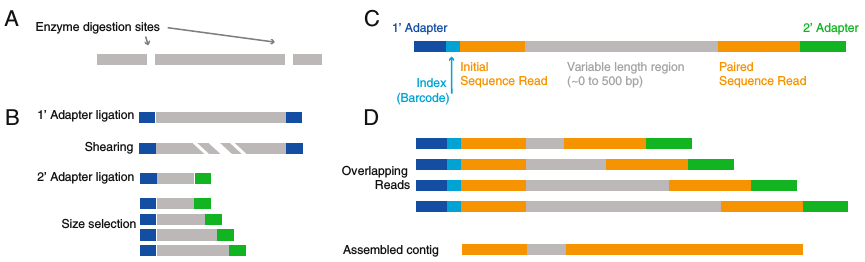
\includegraphics[width=11cm]{Pegadarju2013Fig1.png}



\tiny{\citep{Pegadaraju2013}}
\end{center}
\end{frame}

\begin{frame}[label=sec-1-1-9]{Calling SNPs from RAD-tags}
\begin{center}
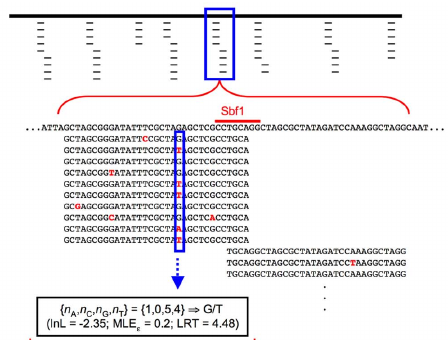
\includegraphics[width=9cm]{HohenloheFig2a.png}



\tiny{\citep{Hohenlohe2010}}
\end{center}
\end{frame}


\begin{frame}[label=sec-1-1-10]{Summary statistics (e.g. population differentiation) along sliding windows}
\begin{center}

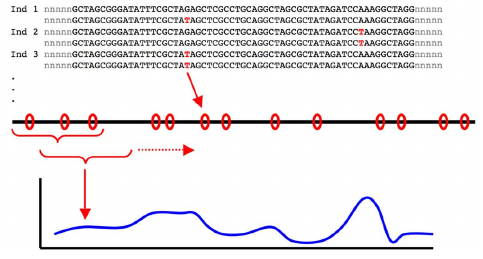
\includegraphics[width=10cm]{HohenloheFig2b.png}

\tiny{\citep{Hohenlohe2010}}
\end{center}
\end{frame}


\begin{frame}[label=sec-1-1-11]{Shearing introduces bias}
 \begin{center}
Bias in sequencing depth towards larger fragment sizes

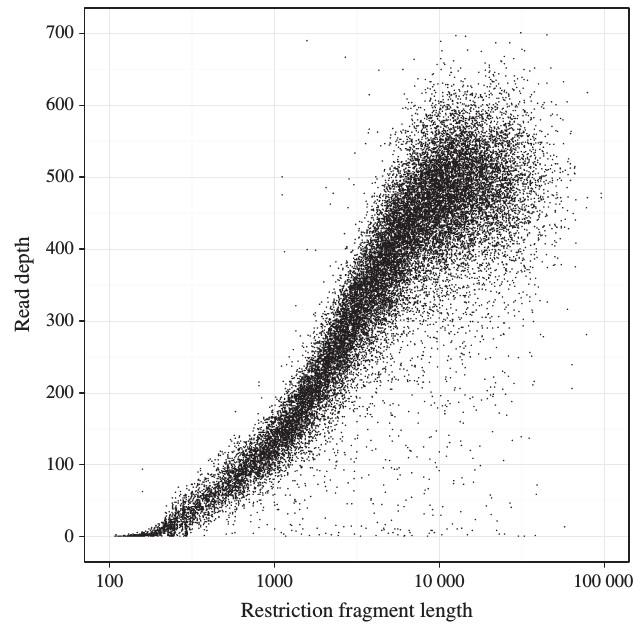
\includegraphics[width=5.5cm]{Davey2013Fig3.png}

 \tiny{\citep{Davey2013}}\\
\normalsize{
Potential reason: Sonicators shear fragments of different lengths with varying efficiencies}

 \end{center}
\end{frame}


\begin{frame}[label=sec-1-1-12]{Amplification bias in favor of high GC content}
 \begin{center}
Read depths are influenced by GC content and number of PCR cycles, with (A) or without  PCR duplicates (B).

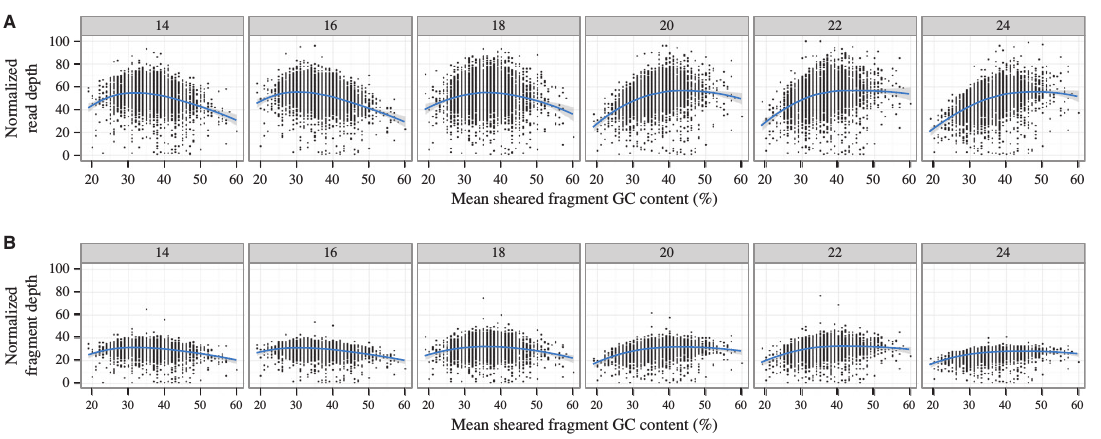
\includegraphics[width=11.5cm]{Davey2013Fig4.png}

 \tiny{\citep{Davey2013}}\\
\normalsize{
Modifications of PCR enrichment can help \tiny{(see \citep{Puritz2014b})}}

 \end{center}
\end{frame}


\section{ddRAD}
\label{sec-2}
\subsection{ddRAD}
\label{sec-2-1}

\begin{frame}[label=sec-2-1-1]{Double-digest RAD-seq \citep{Peterson2012}}
\definecolor{redd}{rgb}{0.8431373,0.09803922,0.1098039}
\definecolor{violet}{rgb}{0.3686275,0.2352941,0.6}
\definecolor{cyan}{rgb}{0,1,1}

\begin{center}

\begin{figure}[htb]
\setlength{\belowcaptionskip}{-1cm}
\scalebox{1}{
\begin{tikzpicture}
\node [anchor=west] at (0cm,0.5cm) {Single digest RAD-Seq}; 
\draw [redd, line width=0.15cm] (0cm,0cm) --  (0.3cm,0cm);
\draw [gray, line width=0.15cm] (0.3cm,0cm) --  (10cm,0cm);
\draw [redd, line width=0.15cm] (1cm,0cm) --  (1.3cm,0cm);
\draw [redd, line width=0.15cm] (5cm,0cm) --  (5.3cm,0cm);
\draw [redd, line width=0.15cm] (7cm,0cm) --  (7.3cm,0cm);
\draw [redd, line width=0.15cm] (10cm,0cm) --  (10.3cm,0cm);


\node [isosceles triangle, draw, rotate=270,scale=0.1,fill=redd!50!black] at (0.05cm,0.2cm) {}; 
\node [isosceles triangle, draw, rotate=90,scale=0.1,fill=redd!50!black] at (0.25cm,-0.2cm) {}; 

\node [isosceles triangle, draw, rotate=270,scale=0.1,fill=redd!50!black] at (1.05cm,0.2cm) {}; 
\node [isosceles triangle, draw, rotate=90,scale=0.1,fill=redd!50!black] at (1.25cm,-0.2cm) {}; 

\node [isosceles triangle, draw, rotate=270,scale=0.1,fill=redd!50!black] at (5.05cm,0.2cm) {}; 
\node [isosceles triangle, draw, rotate=90,scale=0.1,fill=redd!50!black] at (5.25cm,-0.2cm) {}; 

\node [isosceles triangle, draw, rotate=270,scale=0.1,fill=redd!50!black] at (7.05cm,0.2cm) {}; 
\node [isosceles triangle, draw, rotate=90,scale=0.1,fill=redd!50!black] at (7.25cm,-0.2cm) {}; 

\node [isosceles triangle, draw, rotate=270,scale=0.1,fill=redd!50!black] at (10.05cm,0.2cm) {}; 
\node [isosceles triangle, draw, rotate=90,scale=0.1,fill=redd!50!black] at (10.25cm,-0.2cm) {}; 


\draw [violet, line width=0.15cm] (0.55cm,-0.7cm) --  (1.1cm,-0.7cm);
\draw [violet, line width=0.15cm] (0.55cm,-1cm) --  (1.1cm,-1cm);

\draw [violet, line width=0.15cm] (1.2cm,-0.7cm) --  (1.75cm,-0.7cm);
\draw [violet, line width=0.15cm] (1.2cm,-1cm) --  (1.75cm,-1cm);
\draw [violet, line width=0.15cm] (1.2cm,-1.3cm) --  (1.75cm,-1.3cm);


\draw [violet, line width=0.15cm] (4.55cm,-0.7cm) --  (5.1cm,-0.7cm);
\draw [violet, line width=0.15cm] (4.55cm,-1cm) --  (5.1cm,-1cm);
\draw [violet, line width=0.15cm] (4.55cm,-1.3cm) --  (5.1cm,-1.3cm);

\draw [violet, line width=0.15cm] (5.2cm,-0.7cm) --  (5.75cm,-0.7cm);


\draw [violet, line width=0.15cm] (6.55cm,-0.7cm) --  (7.1cm,-0.7cm);
\draw [violet, line width=0.15cm] (6.55cm,-1cm) --  (7.1cm,-1cm);
\draw [violet, line width=0.15cm] (6.55cm,-1.3cm) --  (7.1cm,-1.3cm);

\draw [violet, line width=0.15cm] (7.2cm,-0.7cm) --  (7.75cm,-0.7cm);
\draw [violet, line width=0.15cm] (7.2cm,-1cm) --  (7.75cm,-1cm);

\draw [violet, line width=0.15cm] (9.55cm,-0.7cm) --  (10.1cm,-0.7cm);
\draw [violet, line width=0.15cm] (9.55cm,-1cm) --  (10.1cm,-1cm);


; Second enzyme

\begin{scope}[yshift=-3cm]
\node [anchor=west] at (0cm,0.5cm) {Double digest RAD-seq}; 
\draw [redd, line width=0.15cm] (0cm,0cm) --  (0.3cm,0cm);
\draw [gray, line width=0.15cm] (0.3cm,0cm) --  (10cm,0cm);
\draw [redd, line width=0.15cm] (1cm,0cm) --  (1.3cm,0cm);
\draw [redd, line width=0.15cm] (5cm,0cm) --  (5.3cm,0cm);
\draw [redd, line width=0.15cm] (7cm,0cm) --  (7.3cm,0cm);
\draw [redd, line width=0.15cm] (10cm,0cm) --  (10.3cm,0cm);
\draw [cyan, line width=0.15cm] (1.7cm,0cm) --  (2cm,0cm);
\draw [cyan, line width=0.15cm] (3.5cm,0cm) --  (3.8cm,0cm);
\draw [cyan, line width=0.15cm] (5.5cm,0cm) --  (5.8cm,0cm);
\draw [cyan, line width=0.15cm] (8.5cm,0cm) --  (8.8cm,0cm);


\node [isosceles triangle, draw, rotate=270,scale=0.1,fill=redd!50!black] at (0.05cm,0.2cm) {}; 
\node [isosceles triangle, draw, rotate=90,scale=0.1,fill=redd!50!black] at (0.25cm,-0.2cm) {}; 

\node [isosceles triangle, draw, rotate=270,scale=0.1,fill=redd!50!black] at (1.05cm,0.2cm) {}; 
\node [isosceles triangle, draw, rotate=90,scale=0.1,fill=redd!50!black] at (1.25cm,-0.2cm) {}; 

\node [isosceles triangle, draw, rotate=270,scale=0.1,fill=redd!50!black] at (5.05cm,0.2cm) {}; 
\node [isosceles triangle, draw, rotate=90,scale=0.1,fill=redd!50!black] at (5.25cm,-0.2cm) {}; 

\node [isosceles triangle, draw, rotate=270,scale=0.1,fill=redd!50!black] at (7.05cm,0.2cm) {}; 
\node [isosceles triangle, draw, rotate=90,scale=0.1,fill=redd!50!black] at (7.25cm,-0.2cm) {}; 

\node [isosceles triangle, draw, rotate=270,scale=0.1,fill=redd!50!black] at (10.05cm,0.2cm) {}; 
\node [isosceles triangle, draw, rotate=90,scale=0.1,fill=redd!50!black] at (10.25cm,-0.2cm) {}; 

\node [isosceles triangle, draw, rotate=270,scale=0.1,fill=redd!50!black] at (1.75cm,0.2cm) {}; 
\node [isosceles triangle, draw, rotate=90,scale=0.1,fill=redd!50!black] at (1.95cm,-0.2cm) {}; 

\node [isosceles triangle, draw, rotate=270,scale=0.1,fill=redd!50!black] at (3.55cm,0.2cm) {}; 
\node [isosceles triangle, draw, rotate=90,scale=0.1,fill=redd!50!black] at (3.75cm,-0.2cm) {}; 

\node [isosceles triangle, draw, rotate=270,scale=0.1,fill=redd!50!black] at (5.55cm,0.2cm) {}; 
\node [isosceles triangle, draw, rotate=90,scale=0.1,fill=redd!50!black] at (5.75cm,-0.2cm) {}; 

\node [isosceles triangle, draw, rotate=270,scale=0.1,fill=redd!50!black] at (8.55cm,0.2cm) {}; 
\node [isosceles triangle, draw, rotate=90,scale=0.1,fill=redd!50!black] at (8.75cm,-0.2cm) {}; 

\draw [violet, line width=0.15cm] (4.55cm,-0.7cm) --  (5.1cm,-0.7cm);
\draw [violet, line width=0.15cm] (4.55cm,-1cm) --  (5.1cm,-1cm);
\draw [violet, line width=0.15cm] (4.55cm,-1.3cm) --  (5.1cm,-1.3cm);
\draw [violet, line width=0.15cm] (4.55cm,-1.6cm) --  (5.1cm,-1.6cm);

\draw [violet, line width=0.15cm] (6.55cm,-0.7cm) --  (7.1cm,-0.7cm);
\draw [violet, line width=0.15cm] (6.55cm,-1cm) --  (7.1cm,-1cm);
\draw [violet, line width=0.15cm] (6.55cm,-1.3cm) --  (7.1cm,-1.3cm);

\draw [violet, line width=0.15cm] (7.2cm,-0.7cm) --  (7.75cm,-0.7cm);
\draw [violet, line width=0.15cm] (7.2cm,-1cm) --  (7.75cm,-1cm);
\draw [violet, line width=0.15cm] (7.2cm,-1.3cm) --  (7.75cm,-1.3cm);
\draw [violet, line width=0.15cm] (7.2cm,-1.6cm) --  (7.75cm,-1.6cm);

\draw [violet, line width=0.15cm] (9.55cm,-0.7cm) --  (10.1cm,-0.7cm);
\draw [violet, line width=0.15cm] (9.55cm,-1cm) --  (10.1cm,-1cm);
\draw [violet, line width=0.15cm] (9.55cm,-1.3cm) --  (10.1cm,-1.3cm);

\node [anchor=west] at (0cm,-1.6cm) {Sequencing of fragments:}; 
\node [anchor=west] at (0cm,-2.1cm) {- within a specific size range}; 
\node [anchor=west] at (0cm,-2.6cm) {- flanked by two different cutting sites}; 

\draw [redd, line width=0.15cm] (0.5cm,-3.1cm) --  (0.8cm,-3.1cm);
\draw [cyan, line width=0.15cm] (0.5cm,-3.5cm) --  (0.8cm,-3.5cm);

\node [anchor=west] at (1cm,-3.1cm) {EcoRI recognition site}; 
\node [anchor=west] at (1cm,-3.5cm) {SbfI recognition site}; 

\end{scope}


\end{tikzpicture}
}
\end{figure}
\end{center}
\end{frame}


\begin{frame}[label=sec-2-1-2]{ddRAD compared to single-digest RAD sequencing}
\begin{enumerate}
\item <1> Rapid and 'cheap' protocol (8 hrs hands-on): Doesn't require
difficult and high cost of shearing and enzymatic end-repair.
\item <2> Lower number of loci but increased coverage and, thus, higher
chance to target the same loci in different individuals.
\item <3> Coverage expected to be equal among individuals and highest for
fragment lengths targeted by size selection.
\item <4> Combinatorial indexing allows to multiplex more individuals (up to
12 barcodes were affordable for single-digest RAD-Seq).
\item <5> PCR duplicates can only be detected with specific adapters \citep{Tin2014,Schweyen2014}
\item <6> Precise size selection reduces amplification bias (Pippin Prep
instrument - Sage Science) \citep{Dacosta2014}.
\item <7> Null alleles, which can inflate homozygosity (underestimate
diversity) by allele-dropout, are more frequent in ddRAD (two
recognition sites) \citep{Arnold2013}.
\end{enumerate}
\end{frame}




\begin{frame}[label=sec-2-1-3]{Combinatorial indexing allows for high multiplexing levels in ddRAD-Seq}


\definecolor{adapterp1}{rgb}{0.8431373,0.09803922,0.1098039}
\definecolor{violet}{rgb}{0.3686275,0.2352941,0.6}
\definecolor{adapterp2}{rgb}{0, 0 , 0.803922}
\definecolor{barcode1}{rgb}{0.498039,1,0}
\definecolor{barcode2}{rgb}{1, 0.647059, 0}
\definecolor{barcode4}{rgb}{0.196078, 0.803922, 0.196078}
\definecolor{sequencingprimer}{rgb}{0.9882353,0.5529412,0.3490196}
\definecolor{amplificationprimer}{rgb}{0.2705882,0.4588235,0.7058824}





\begin{center}
\begin{figure}[htb]
\setlength{\belowcaptionskip}{-1cm}
\scalebox{1}{
\begin{tikzpicture}
\draw [violet, line width=0.2cm] (0cm,0cm) --  (1cm,0cm);
\draw [violet, line width=0.2cm] (9cm,0cm) --  (10cm,0cm);
\draw [adapterp1, line width=0.2cm] (1cm,0cm) --  (2cm,0cm);
\draw [adapterp2, line width=0.2cm] (7.6cm,0cm) --  (8.6cm,0cm);
\draw [barcode2, line width=0.2cm] (2cm,0cm) --  (2.4cm,0cm);
\draw [barcode4, line width=0.2cm] (8.6cm,0cm) --  (9cm,0cm);


\draw [gray, line width=0.2cm] (2.4cm,0cm) --  (7.6cm,0cm);

\node [barcode2,anchor=west] at (2cm, -1cm){Inline barcode (sequenced)};
\node [adapterp1,anchor=west] at (1cm, -1.5cm){Adapter P1};
\node [violet,anchor=west] at (0cm, -2cm){Flowcell annealing};


\node [adapterp2,anchor=east] at (8.6cm, 1cm){Adapter P2};
\node [barcode4,anchor=east] at (9cm, 1.5cm){Index adapter (Illumina)};
\node [violet,anchor=east] at (10cm, 2cm){Flowcell annealing};

\draw (0.5,-0.3cm) -- (0.5,-1.7cm);
\draw (1.5,-0.3cm) -- (1.5,-1.3cm);
\draw (2.2,-0.3cm) -- (2.2,-0.7cm);

\draw (9.5,0.3cm) --  (9.5,1.7cm);
\draw (8.8,0.3cm) -- (8.8,1.3cm);
\draw (8.1,0.3cm) --  (8.1,0.7cm);

\node [barcode2,anchor=west] at (0cm, -2.8cm){48};
\node [anchor=west] at (0.6cm, -2.8cm){x};
\node [barcode4,anchor=west] at (1cm, -2.8cm){12};
\node [anchor=west] at (1.5cm, -2.8cm){= 576 (multiplexing level)};

\node [barcode2,anchor=west] at (0cm, -3.5cm) {added first, with ligation of adapters, allows to pool samples};
\node [barcode4,anchor=west] at (0cm, -4cm) {added second, with PCR primer, allows to combine multiple pools};

\end{tikzpicture}
} 
\end{figure}
\end{center}
\end{frame}
\begin{frame}[label=sec-2-1-4]{Pooling recommendations}
\begin{itemize}
\item Critical: equimolar concentrations of individuals expected
\item Recommended: >40 individuals/pool
\begin{itemize}
\item Higher numbers
\begin{itemize}
\item + decrease unequal representation of individuals in
the pool
\item - make it more more difficult to discriminate minor allele
frequencies from sequencing errors
\end{itemize}
\end{itemize}
\end{itemize}
\end{frame}
\begin{frame}[label=sec-2-1-5]{Great adjustability of the number of markers makes ddRAD suitable for a broader range of approaches than RAD-Seq}
Number of markers adjusted by:
\begin{itemize}
\item Cutting frequency of restriction enzymes
\item Size selection
\end{itemize}
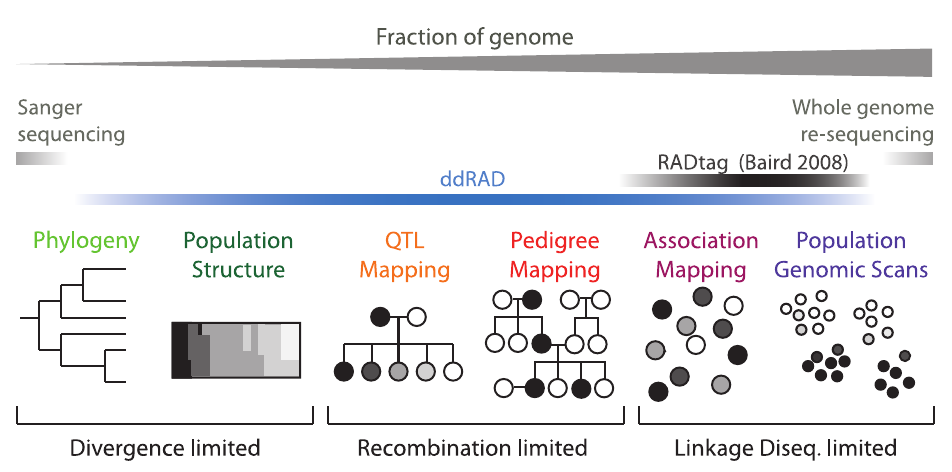
\includegraphics[width=10cm]{Peterson-2012-Fig1.png}   
\begin{center}
\tiny{\citep{Peterson2012}}
\end{center}
\end{frame}
\begin{frame}[label=sec-2-1-6]{How to predict the number of fragments}
Based on our own study on Guppy
\begin{itemize}
\item Targeted coverage: 20x per individual
\item Pooling: 60 individuals
\item Sequencing output: 24M reads (12M fragments, minimum for Illumina v2
paired-end kits)
\item Fragments per individual: 12M/60 = 200,000

\item Target: \alert{10,000} fragments (to reach a 20x coverage)
\end{itemize}

What combination of restriction enzymes to use to obtain the appropriate cutting
frequency?
\end{frame}
\begin{frame}[label=sec-2-1-7]{\emph{In silico} genome digestion}
Simulate restriction enzyme digestion with the R package simRAD \citep{Lepais2014}
\begin{center}
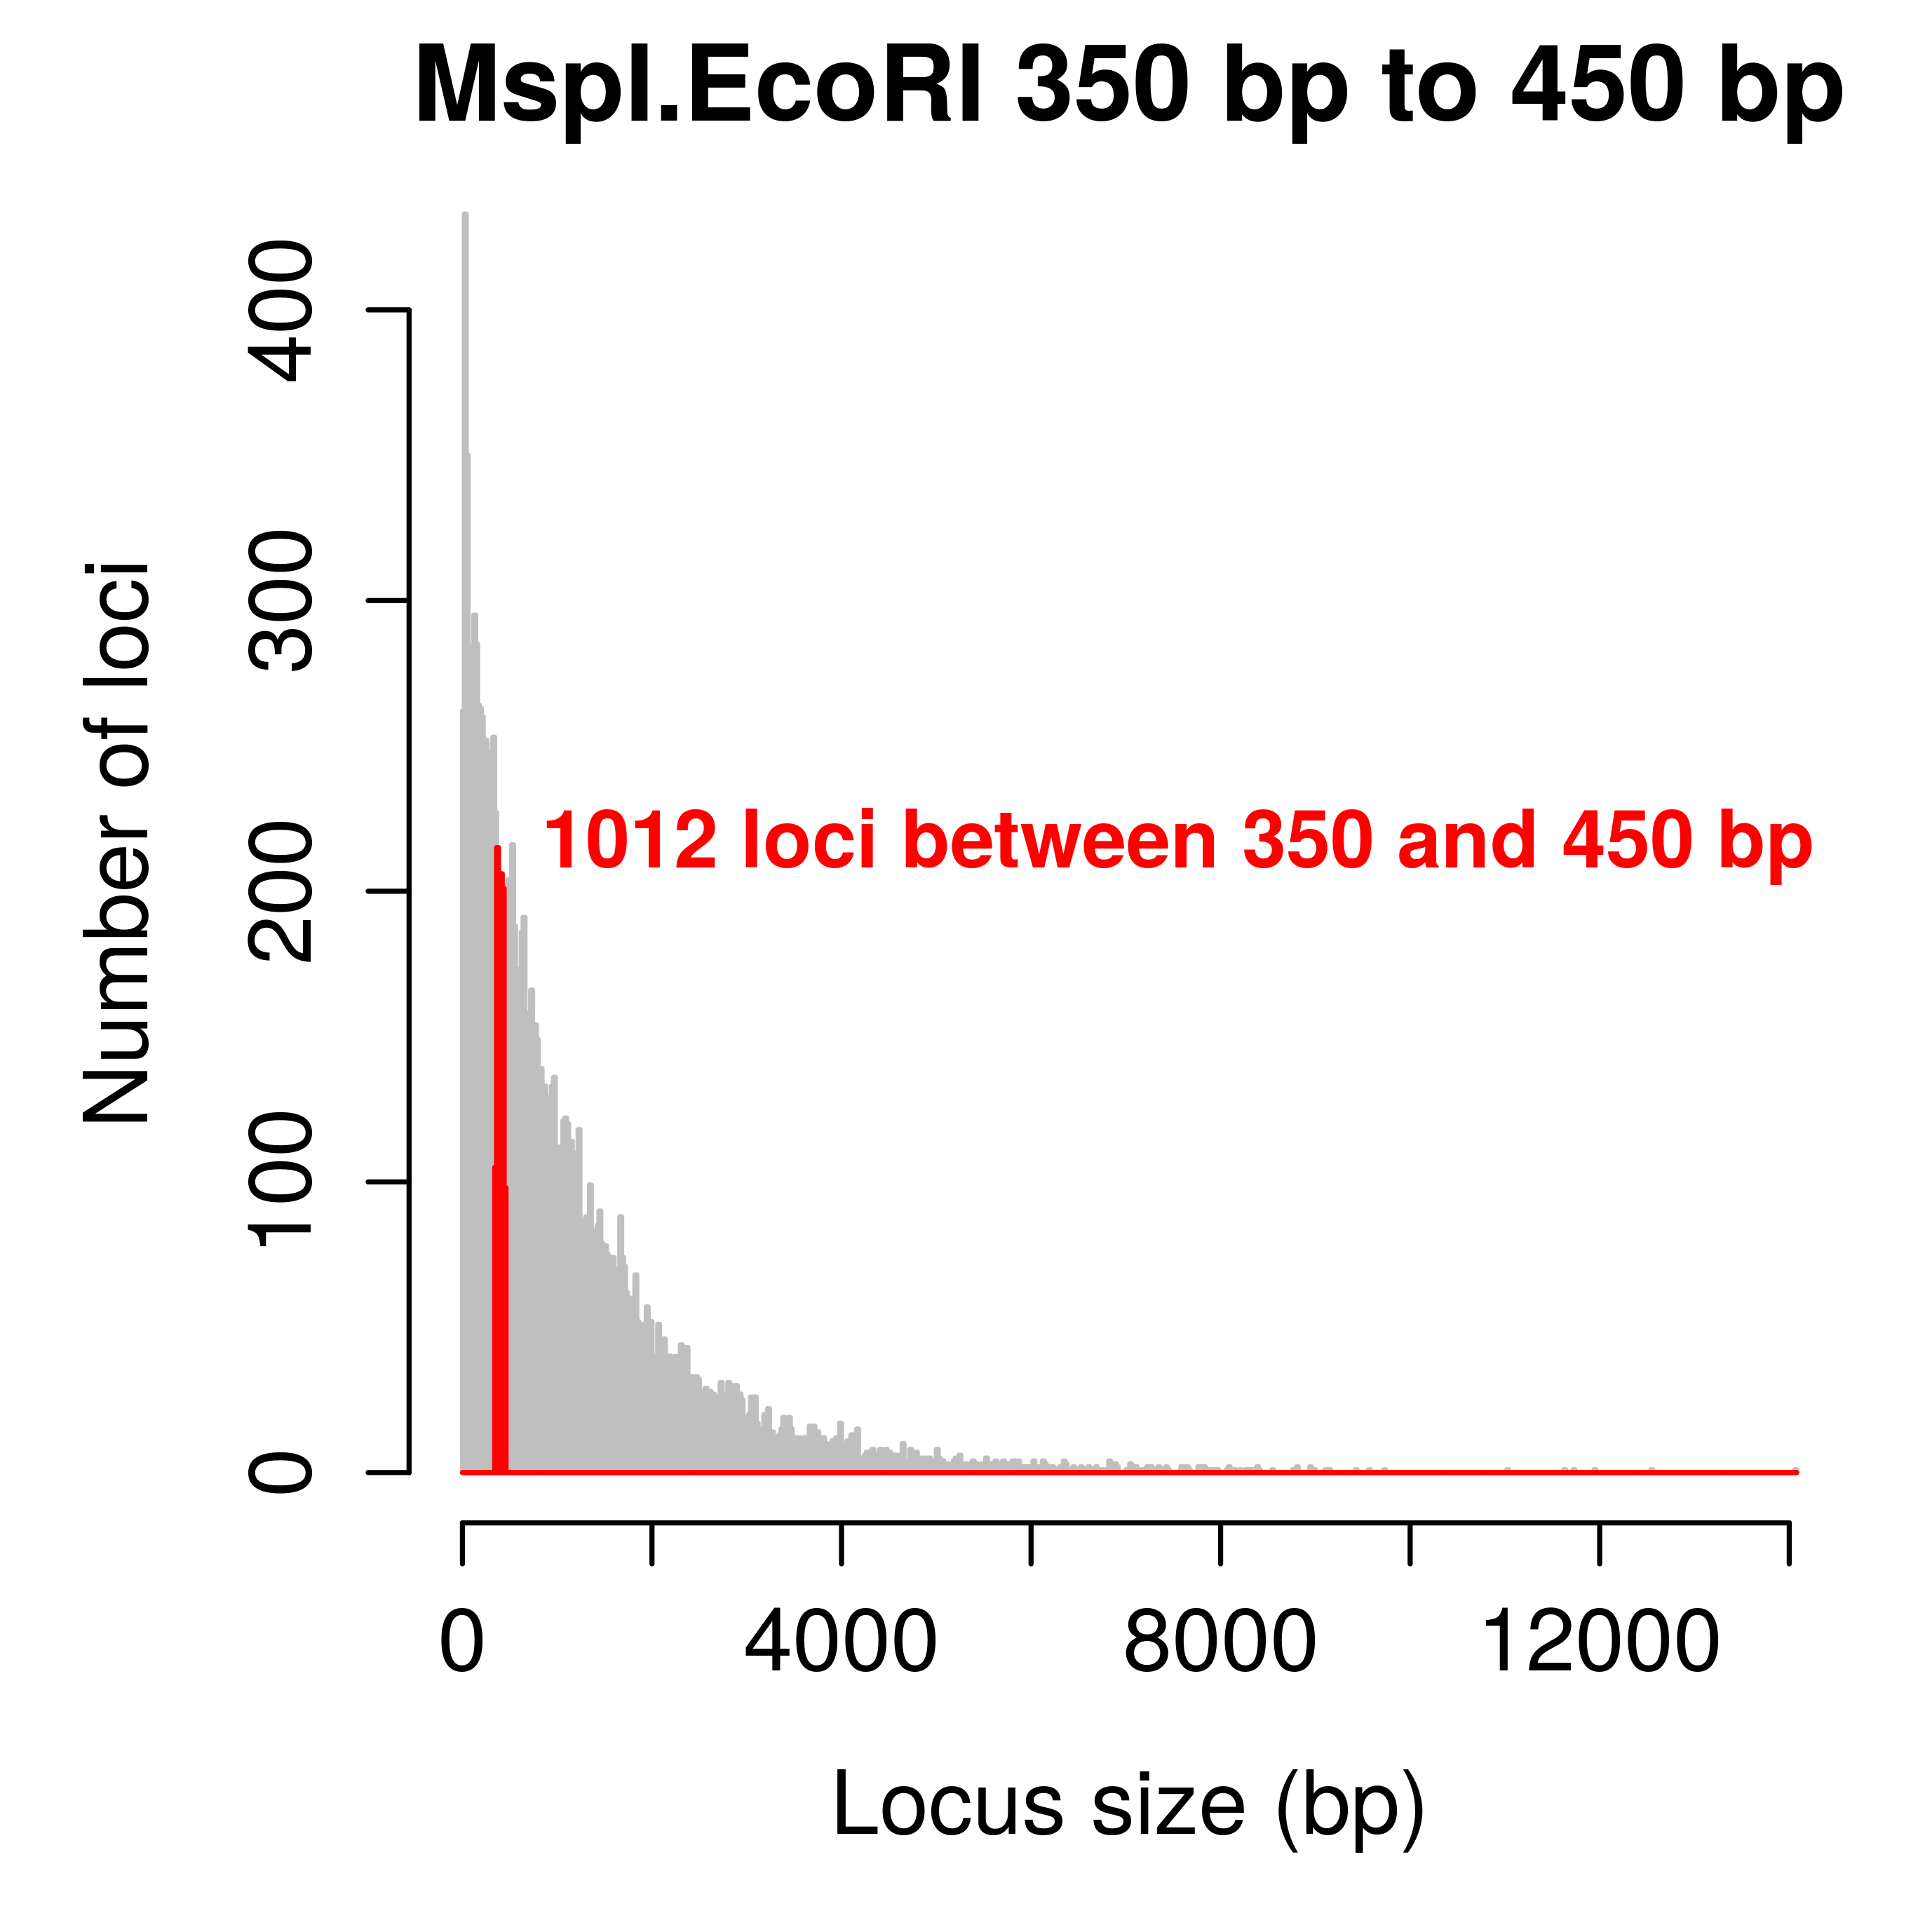
\includegraphics[width=5cm]{MspIEcoRI350to450.png}

\small{Based on 10\% of the entire genome size}
\end{center}
Without reference genome: evaluate double-digest fragments on Tape station
\end{frame}


\begin{frame}[label=sec-2-1-8]{Recovery of \emph{in silico} predicted loci}
\begin{center}
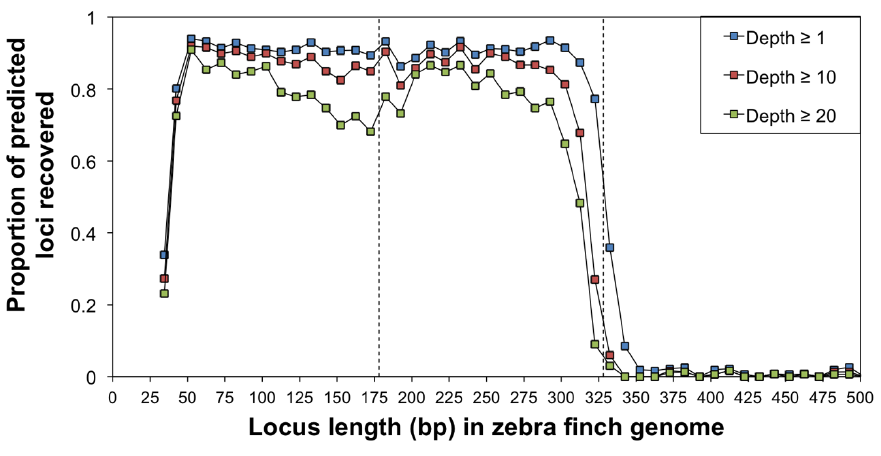
\includegraphics[width=9cm]{DaCosta2014Fig1a.png}

 \tiny{\citep{Dacosta2014}}\\
\small{Targeted: 178-328bp, but short restriction fragments (38–178 bp) were carried through the agarose gel size selection step}
 \end{center}
\end{frame}

\begin{frame}[label=sec-2-1-9]{Sequencing depth decreases with fragment lenth}
\begin{center}
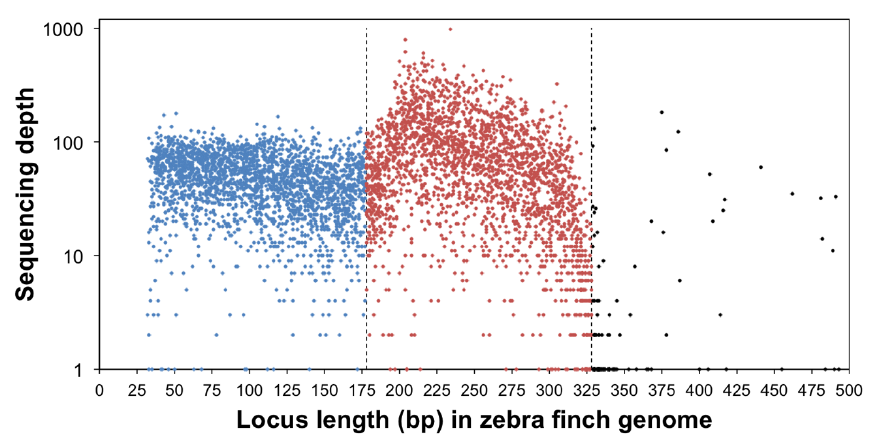
\includegraphics[width=9.5cm]{DaCosta2014Fig1b.png}

\tiny{\citep{Dacosta2014}}
\end{center}
\begin{itemize}
\item Opposite to RADseq (shearing bias)
\item Negative correlation between depth and fragment length in the 178–200 bp range, not for smaller loci.
\item Among-locus variation in sequencing depth was consistent among samples.
\end{itemize}
\end{frame}

\begin{frame}[label=sec-2-1-10]{Sequencing depth bias in favor of loci with high GC content}
\begin{center}
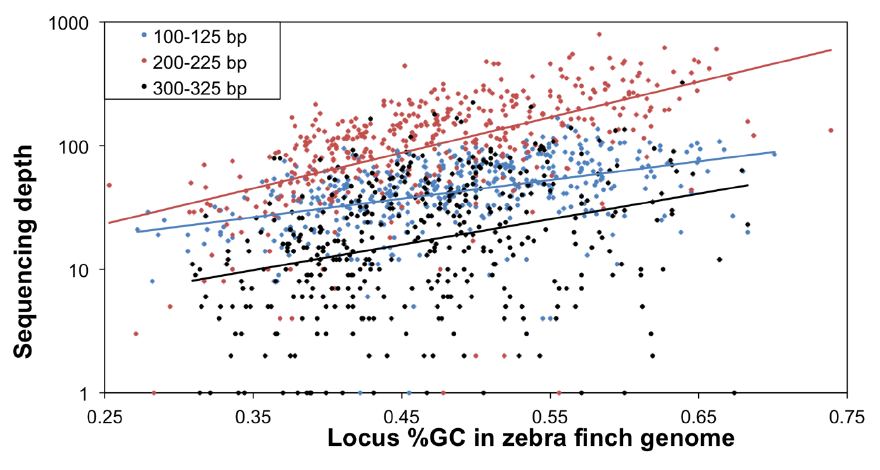
\includegraphics[width=10cm]{DaCosta2014Fig1c.png}

\tiny{\citep{Dacosta2014}}
\end{center}
\begin{itemize}
\item Combined with a GC-rich recognition sequence, this can result
in an overrepresentation of GC-rich portions of the genome
\end{itemize}
\end{frame}

\begin{frame}[label=sec-2-1-11]{PCR duplicates}
\begin{itemize}
\item PCR duplicates are statistically nonindependent and inflate the
confidence of genotype calls at a site.
\item Can inflate the proportion of homozygous loci (allele dropout)
\citep{Schweyen2014}.
\item RAD-tags: homologous sequences start at the same location and can
not be discriminated from PCR duplicates if they have the same
length. All are generally removed
\item ddRAD-tags: Paired-end sequences always start and end at the same
position
\item Detection of duplicate reads only possible with specific adapters of
random four bases that are ligated to the first index read of the
template molecule before PCR. \citep{Tin2014,Schweyen2014}.
\end{itemize}
\end{frame}
\begin{frame}[label=sec-2-1-12]{Detect PCR duplicates in paired-end RAD sequencing}
\vspace{0.1cm}

\begin{columns}
\begin{column}{0.3\columnwidth}
\begin{raggedright}
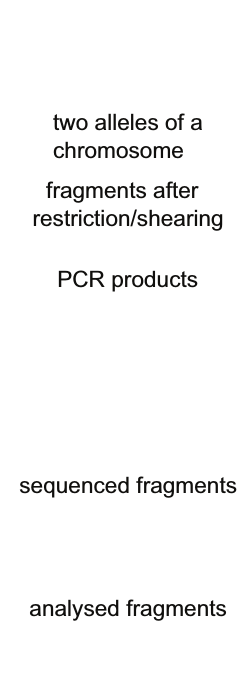
\includegraphics[width=2.8cm]{Schweyen2014Fig2a.png}
\end{raggedright}
\end{column}

\begin{column}{0.3\columnwidth}
\begin{raggedleft}
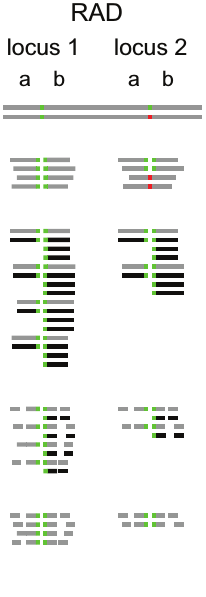
\includegraphics[width=2.8cm]{Schweyen2014Fig2b.png}
\end{raggedleft}
\end{column}
\begin{column}{0.3\columnwidth}
\begin{raggedleft}
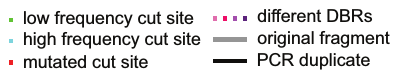
\includegraphics[width=3.5cm]{Schweyen2014Fig2e.png}
\end{raggedleft}
\tiny{\citep{Schweyen2014}}\\
PCR bias amplifies b more than a
\end{column}
\end{columns}
\end{frame}

\begin{frame}[label=sec-2-1-13]{PCR duplicates in ddRAD - not detectable}
\vspace{0.1cm}

\begin{columns}
\begin{column}{0.3\columnwidth}
\begin{raggedright}
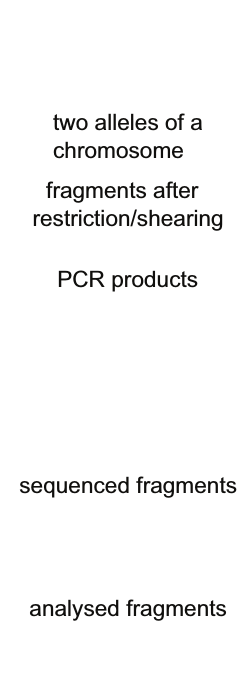
\includegraphics[width=2.8cm]{Schweyen2014Fig2a.png}
\end{raggedright}
\end{column}

\begin{column}{0.3\columnwidth}
\begin{raggedleft}
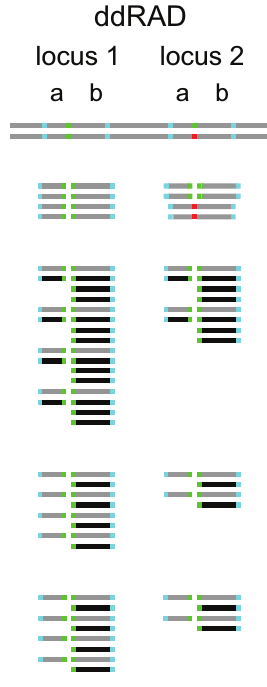
\includegraphics[width=2.8cm]{Schweyen2014Fig2c.png}
\end{raggedleft}
\end{column}
\begin{column}{0.3\columnwidth}
\begin{raggedleft}
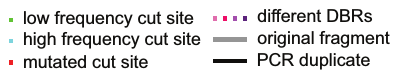
\includegraphics[width=3.5cm]{Schweyen2014Fig2e.png}
\end{raggedleft}
\tiny{\citep{Schweyen2014}}\\
locus 2 with mutated cut site can have equal coverage as locus 1
\end{column}
\end{columns}
\end{frame}
\begin{frame}[label=sec-2-1-14]{Degenerate base regions detect PCR duplicates in ddRAD}
\vspace{0.1cm}

\begin{columns}
\begin{column}{0.3\columnwidth}
\begin{raggedright}
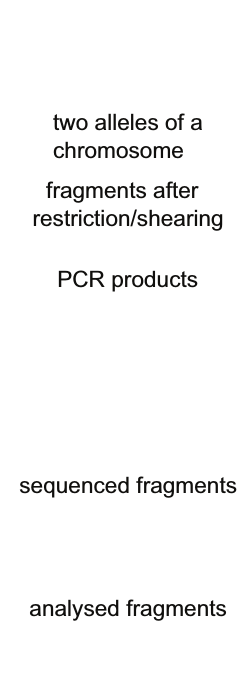
\includegraphics[width=2.8cm]{Schweyen2014Fig2a.png}
\end{raggedright}
\end{column}

\begin{column}{0.3\columnwidth}
\begin{raggedleft}
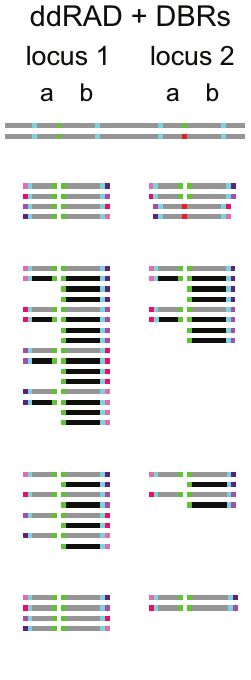
\includegraphics[width=2.8cm]{Schweyen2014Fig2d.png}
\end{raggedleft}
\end{column}

\begin{column}{0.3\columnwidth}
\begin{raggedleft}
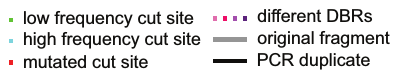
\includegraphics[width=3.5cm]{Schweyen2014Fig2e.png}
\end{raggedleft}
\tiny{\citep{Schweyen2014}}
\end{column}
\end{columns}
\end{frame}

\section{Pipelines}
\label{sec-3}
\subsection{Pipelines}
\label{sec-3-1}
\begin{frame}[label=sec-3-1-1]{STACKS - basic pipeline for RAD-Seq}
\begin{center}
STACKS - software pipleine to build loci from RADseq reads and use
them for population genomics and phylogeographic analyses.

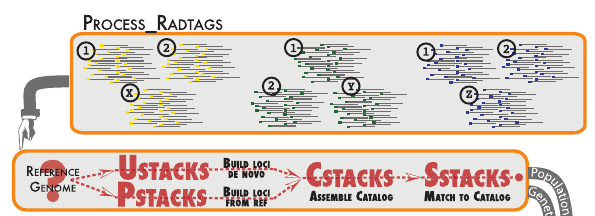
\includegraphics[width=10cm]{Catchen2013Fig1a.png}

\tiny{\citep{Catchen2013a}}
\end{center}
\end{frame}


\begin{frame}[label=sec-3-1-2]{STACKS - ustacks \emph{de novo} assembly step 1}
\begin{itemize}
\item Only exact matches are assembled
\item Secondary reads are set aside
\item The minimum stack depth parameter controls the number of raw reads  required to form an initial stack
\begin{center}
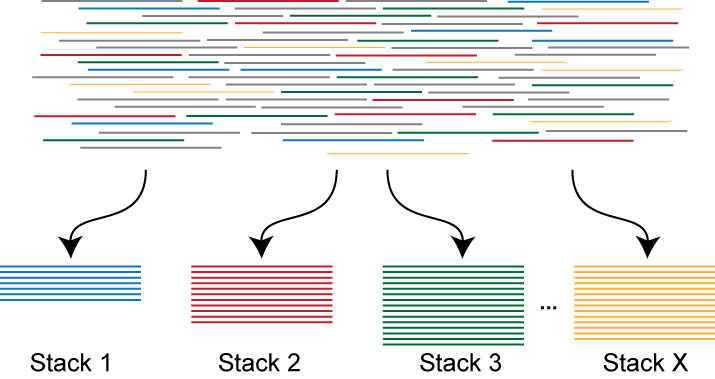
\includegraphics[width=9cm]{Catchen2013DeNovoStep1.png}

\tiny{\citep{Catchen2013a}}
\end{center}
\end{itemize}
\end{frame}




\begin{frame}[label=sec-3-1-3]{STACKS - Ustacks \emph{de novo} assembly step 2}
\begin{itemize}
\item Stacks with few nucleotide differences are merged.
\item Repetitive sequences with many alleles are excluded
\begin{center}
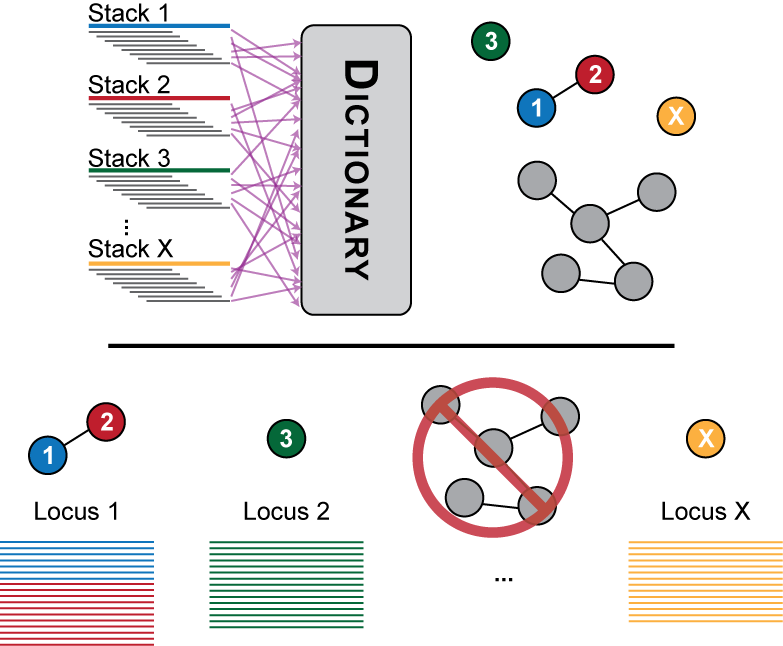
\includegraphics[width=8cm]{Catchen2013DeNovoStep2.png}

\tiny{\citep{Catchen2013a}}
\end{center}
\end{itemize}
\end{frame}


\begin{frame}[label=sec-3-1-4]{STACKS - Ustacks \emph{de novo} assembly step 3}
\begin{itemize}
\item Alignment of secondary reads (those not indcluded in stacks) against
stacks.
\item Alleles are discriminated from sequencing errors by their frequency.
\begin{center}
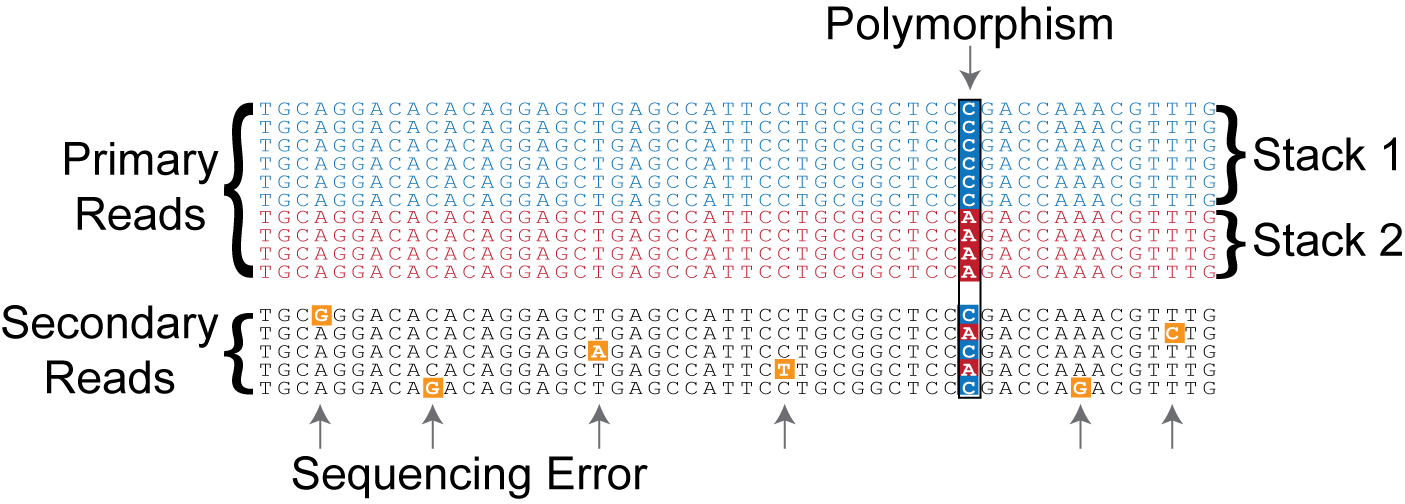
\includegraphics[width=10cm]{Catchen2013DeNovoStep3.png}

\tiny{\citep{Catchen2013a}}
\end{center}
\end{itemize}
\end{frame}

\begin{frame}[label=sec-3-1-5]{STACKS - populations or genotypes pipeline}
\begin{center}
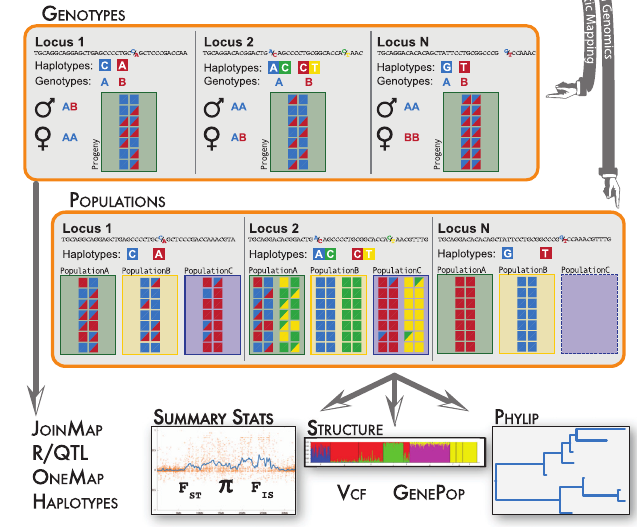
\includegraphics[width=9cm]{Catchen2013Fig1b.png}

\tiny{\citep{Catchen2013a}}
\end{center}
\end{frame}


\begin{frame}[label=sec-3-1-6]{DDocent \citep{Puritz2014}}
Uses stand-alone software packages to perform
\begin{itemize}
\item quality trimming
\item adapter removal
\item \emph{de novo} assembly of RAD loci
\item read mapping
\item SNP and InDel calling
\item data filtering.
\end{itemize}

Identifies more SNPs at a higher coverage than STACKS, due to 
\begin{itemize}
\item simulatneous use of forward and reverse reads during alignment to
reference instead of clustering
\item quality trimming instead of removing entire reads
\end{itemize}
\end{frame}

\section{ezRAD and 2bRAD}
\label{sec-4}

\subsection{ezRAD and 2bRAD}
\label{sec-4-1}

\begin{frame}[label=sec-4-1-1]{ezRAD \citep{Toonen2013}}
\begin{itemize}
\item Uses 2 isoschizomers of restriction enzymes specific to the same recognition sequence (GATC)
\item digested DNA is inserted in Illumina TruSeq library preparation kit.
\item DNA is digested and single- or dual-indexed, then pooled and size-selected.
\end{itemize}
\begin{block}{Advantages}
\begin{itemize}
\item non-PCR kits can avoid PCR duplication and bypass any PCR bias.
\end{itemize}
\end{block}
\begin{block}{Disadvantages}
\begin{itemize}
\item All reads start with the same four bases (GATC).
\begin{itemize}
\item Low diversity libraries can lead to poor read quality on Illumina
sequencers. Use e.g. PhiX spiking or dark-cycling.
\end{itemize}
\end{itemize}
\end{block}
\end{frame}



\begin{frame}[label=sec-4-1-2]{2bRAD \citep{Wang2012}}
\begin{itemize}
\item Type IIb restriction endonuclease to excise 36-bp fragments.
\item Number of loci customized by base-selective adapters.
\end{itemize}

\begin{center}
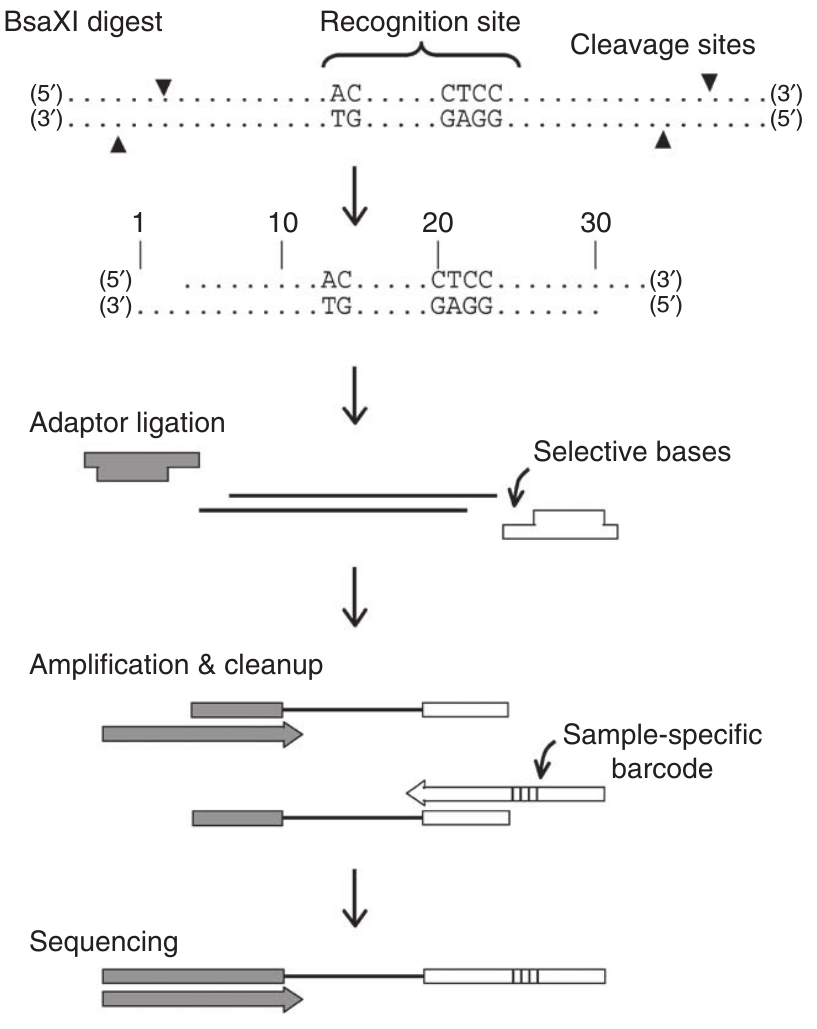
\includegraphics[width=5cm]{Wang2012Fig1.png}


\tiny{\citep{Wang2012}}
\end{center}
\end{frame}

\begin{frame}[label=sec-4-1-3]{2bRAD \citep{Wang2012}}
\begin{block}{Advantages}
\begin{itemize}
\item Extremely simple and cost-effective: no purification or size selection.
\item No biases due to fragment size selection.
\item Sequencing either strand of the restriction fragments allows for the
use of strand bias as a quality filtering criteria.
\end{itemize}
\end{block}
\begin{block}{Disadvantages}
\begin{itemize}
\item 36-bp tags could be too short to be non-ambiguously mapped in highly
duplicated genomes.
\item Likely not cross-mappable across large genetic distances.
\end{itemize}
\end{block}
\end{frame}

\begin{frame}[allowframebreaks]{References}
\raggedright
\printbibliography[sorting=nty,heading=bibnumbered]
\end{frame}
% Emacs 24.3.1 (Org mode 8.3beta)
\end{document}